\documentclass[dvipsnames, svgnames, x11names]{beamer}
\usetheme{mytheme2024}
% \special{dvipdfmx:config z 0} %取消PDF压缩，加快速度，最终版本生成的时候最好把这句话注释掉

\title{化学反应工程}
\subtitle{多相系统中的化学反应与传递现象}
\author{张斌}
\institute[理工系]{河北农业大学 理工系}
\date{\the\year 年 \the\month 月}
%-----------------------------------------------------------------
\begin{document}

\maketitle


\begin{frame}
    \frametitle{多相系统}

    实际生产中，多数化学反应系在多相系统中进行。多相系统的特征是系统中同时存在两个或两个以上的相态，所以，与发生化学反应的同时，必然伴随着相间和相内的传递现象，这主要是质量传递和热量传递。

    根据化学反应进行的部分，可将多相系统概括为三种基本类型：
    \begin{itemize}
        \item 在两相界面处进行反应
        
        所有气固反应或气固相催化反应都属于这一类型；
        \item 在一个相内进行反应
        
        大多数气液反应均属于这种情况，即反应都是在液相中进行的，进行反应的相叫做反应相；
        \item 在两个相内同时发生反应
        
        某些液液反应属于这种情况。
    \end{itemize}

\end{frame}



\begin{frame}{}
    \begin{center}
        {\Huge \cbf{目 \ 录}}
    \end{center}
    \tableofcontents
    \thispagestyle{empty}
    \addtocounter{framenumber}{-1}
\end{frame}


\section{多相催化反应步骤}


\begin{frame}
    \frametitle{气固相催化反应过程步骤}

    \begin{minipage}{0.46\linewidth}
        
\includegraphics[width=\linewidth]{figures/fig6.1.png}
    \end{minipage}\hfill
    \begin{minipage}{0.52\linewidth}
        \begin{enumerate}
            \item 反应物A由气相主体扩散到颗粒外表面；
            \item 反应物A由外表面向孔内扩散，到达可进行吸附/反应的活性中心；
            \item A的吸附
            \item A在表面上反应生成B
            \item 产物B自表面解吸
            \item 产物B由内表面扩散到外表面；
            \item B由颗粒外表面扩散到气相主体
        \end{enumerate}
    \end{minipage}
    \bigskip

    3、4、5总称为表面反应过程，其反应历程就决定了该催化反应的本征动力学。

\end{frame}


\begin{frame}
    \frametitle{气固相催化反应过程步骤}

    \begin{minipage}{0.46\linewidth}
        
\includegraphics[width=\linewidth]{figures/fig6.1.png}
    \end{minipage}\hfill
    \begin{minipage}{0.52\linewidth}
        由于扩散的影响，流体主体、催化剂外表面及催化剂颗粒中心反应物的浓度$c_\mathrm{AG}$、$c_\mathrm{AS}$和$c_\mathrm{AC}$将是不一样的。$c_\mathrm{Ae}$为平衡浓度。
        \begin{itemize}
            \item $c_\mathrm{AG} > c_\mathrm{AS} > c_\mathrm{AC} > c_\mathrm{Ae}$
        \end{itemize}
        对于反应产物，浓度高低顺序相反
        \begin{itemize}
            \item $c_\mathrm{BG} < c_\mathrm{BS} < c_\mathrm{BC} < c_\mathrm{Be}$
        \end{itemize}
    \end{minipage}

\end{frame}


\begin{frame}
    \frametitle{固体催化剂}

    绝大多数固体催化剂颗粒为多孔结构，即颗粒内部系由许许多多形状不规则互相连通的孔道所组成，形成一几何形状复杂的网络结构。正是由于这种网状结构的存在，使催化剂颗粒内部存在着巨大的表面，化学反应便是在这些表面上发生的。通常以\highlight{比表面}来衡量催化剂表面的大小，以\si{m^2/g}为单位。

    \begin{figure}[htpb]
        \centering
        \setcounter{subfigure}{0}
        \subfloat[活性炭催化剂]{
\includegraphics[height=3.7cm]{C}}\quad
        \subfloat[氧化铝催化剂]{
\includegraphics[height=3.7cm]{Al2O3}}
    \end{figure}

\end{frame}


\begin{frame}
    \frametitle{固体催化剂的结构性质}
    \begin{enumerate}
      \item 孔容：单位质量催化剂颗粒所具有的孔体积，\si{cm^3/g}
      \item 平均孔半径：
      \item 孔隙体积与催化剂颗粒体积之比
      \item 当量直径：形状不规则的颗粒，用与颗粒相当的球体直径来表示颗粒的粒度
      \item 形状系数：与球形相接近的程度
    \end{enumerate}
\end{frame}


\begin{frame}
    \frametitle{孔容}

    多孔催化剂的比表面显然与孔道的大小有关，孔道越细，则比表面越大。然而催化剂颗粒内的孔道又是粗细不一的，通常用孔径分布来描述，孔径分布则是通过由实验测定的孔容分布计算得到。
    
    孔容是指单位质量催化剂颗粒所具有的孔体积，常以\si{cm^3/g}为单位。
    \begin{itemize}
        \item 可用压汞仪来测定不同大小的孔的体积
        
        可以测出较宽范围的孔径分布，测试孔径范围约为 \SI{3}{nm} $\sim 360 \mu$m
        \item 四氯化碳法测定催化剂的孔容
        
        测得的孔体积包括所有孔的体积，或称总孔容，通常所说的孔容指的就是总孔容。
    \end{itemize}

\end{frame}


\begin{frame}
    \frametitle{平均孔半径}

    为了定量比较和计算上的方便，常用平均孔半径$\langle r_\mathrm{a} \rangle$来表示催化剂孔的大小。如果不同孔径$r_\mathrm{a}$的孔容分布已知，平均孔径$\langle r_\mathrm{a} \rangle$可由下式算出
    \[
        \langle r_\mathrm{a} \rangle = \frac{1}{V_\mathrm{g}} \int_0^{V_\mathrm{g}} r_\mathrm{a} \dif V
    \]
    式中$V$为半径为$r_\mathrm{a}$的孔的体积，按单位质量催化剂计算，$V_\mathrm{g}$为催化剂总孔容。缺乏孔容分布数据时，只要催化剂的比表面$S_\mathrm{g}$及总孔容已知，也可按下列办法估算平均孔径。
    \[
        \langle r_\mathrm{a} \rangle = 2V_\mathrm{g}/S_\mathrm{g}
    \]

\end{frame}


\begin{frame}
    \frametitle{孔隙率}

    除了用孔容来表示催化剂颗粒的孔体积外，还可用孔隙率（或简称孔率）$\varepsilon_\mathrm{p}$来表示。孔隙率等于孔隙体积与催化剂颗粒体积（固体体积与孔隙体积之和）之比，显然$\varepsilon_\mathrm{p} < 1$。孔率与孔容的差别在于前者按单位颗粒体积，而后者则是按单位质量催化剂计算的孔体积。两者的关系为
    \[
        \varepsilon_\mathrm{p} = V_\mathrm{g} \rho_\mathrm{p}
    \]
    式中$\rho_\mathrm{p}$为颗粒密度，或称表观密度。除了颗粒密度之外，还有所谓真密度$\rho_\mathrm{t}$和堆密度$\rho_\mathrm{b}$，它们的定义可分别表示如下
    \[
        \rho_\mathrm{p} = \frac{\text{固体的质量}}{\text{颗粒的体积}} \qquad \rho_\mathrm{t} = \frac{\text{固体的质量}}{\text{固体的体积}} \qquad \rho_\mathrm{b} = \frac{\text{固体的质量}}{\text{床层的体积}}
    \]

\end{frame}


\begin{frame}[t]
    \frametitle{}

    \begin{block}{例6.1}
        已知一催化剂颗粒的质量为\SI{1.2}{g}，体积为\SI{1}{cm^3}，测得孔容为\SI{0.25}{cm^3/g}，比表面为 \SI{100}{m^2/g}，试求这粒催化剂的$\rho_\mathrm{p}$、$\varepsilon_\mathrm{p}$及$\langle r_\mathrm{a} \rangle$。
    \end{block}
    \pause
    \[
        \begin{aligned}
            \rho_\mathrm{p} &= 1.2/1 = 1.2 \ \si{g/cm^{3}} \\
            \varepsilon_\mathrm{p} &= 0.25\times 1.2 = 0.3 \\
            \langle r_\mathrm{a} \rangle &= 2V_\mathrm{g}/S_\mathrm{g} = 2\times 0.25\times 10^{-4}/100  = 5\times 10^{-7} \ \mathrm{cm}
        \end{aligned}
    \]
\end{frame}


\begin{frame}
    \frametitle{颗粒粒度的表示方法：当量直径}

    对于固体颗粒，尤其是形状不规则而又较细的颗粒，往往通过筛分来确定其粒度，例如40、60目的颗粒，意指这些颗粒能通过40目筛，而不能通过60目筛。同时以这两种筛的筛孔净宽的算术平均值来表示颗粒的线性尺寸。
    
    \bigskip

    在实际设计计算中，往往以与颗粒相当的球体直径来表示颗粒的粒度，具体做法有三种。
    
    \only<1>{
            \begin{enumerate}
        \item 以与颗粒体积相等的球体直径表示；
        \item 以与颗粒外表面积相等的球体直径表示；
        \item 以与颗粒的比外表面积相等的球体直径表示。
    \end{enumerate}
    }
    \only<2>{
            \begin{enumerate}
        \item 以与颗粒体积相等的球体直径表示；$V = \frac{4}{3}\pi r_\mathrm{p}^3 \qquad d_{V} = \sqrt[3]{\frac{6V}{\pi}}$
        \item 以与颗粒外表面积相等的球体直径表示；$S = 4\pi r_\mathrm{p}^2 \qquad d_S = \sqrt{\frac{S}{\pi}}$
        \item 以与颗粒的比外表面积相等的球体直径表示。$\frac{S}{V_\mathrm{p}} = \frac{3}{r_\mathrm{p}} \qquad d_{SV} = \frac{6V}{S}$
    \end{enumerate}
    }

\end{frame}


\begin{frame}
    \frametitle{颗粒外形与球形接近的程度：形状系数}

    形状系数$\phi_\mathrm{a}$的意义为和颗粒体积相同的球体的外表面积$a_\mathrm{s}$与颗粒的外表面积$a_\mathrm{p}$之比，即
    \[
        \phi_\mathrm{a} = a_\mathrm{s} / a_\mathrm{p}
    \]
    由于体积相同的几何体中以球体的外表面积为最小，所以$a_\mathrm{s} < a_\mathrm{p}$，$\phi_\mathrm{a} < 1$。
    
    $\phi_\mathrm{a} = 1$表明颗粒为球形。
    
    $\phi_\mathrm{a}$表示颗粒外形与球形相接近的程度，又称圆球度。

\end{frame}


\section{流体与催化剂颗粒外表面的传质与传热}


\begin{frame}
    \frametitle{流体与催化剂颗粒外表面的传质}

    多相催化反应过程的第一步是反应物向催化剂颗粒外表面传递，这一步骤的速率可用下式来表示
    \[
        N_{\mathrm{A}} =k_{\mathrm{G}} a_{\mathrm{m}}(c_{\mathrm{AG}}-c_{\mathrm{AS}})
    \]
    式中$a_{\mathrm{m}}$为单位质量催化剂颗粒的外表面积，$k_{\mathrm{G}}$为传质系数。
    
    浓度差$(c_{\mathrm{AG}}-c_{\mathrm{AS}})$为传质过程推动力。
    
    对于定态过程，这一传质速率应等于反应物A的转化速率$-\mathscr{R}_{\mathrm{A}}$，即
    \[
        N_{\mathrm{A}} = -\mathscr{R}_{\mathrm{A}}
    \]

\end{frame}


\begin{frame}
    \frametitle{流体与催化剂颗粒外表面的传热}

    由于化学反应进行时总是伴随着一定的热效应，放热或吸热，因而在反应物向催化剂颗粒外表面传递的同时，必然产生流体与颗粒外表面间的热量传递，进行放热反应时，热量从催化剂外表面向流体主体传递，吸热反应则相反，此传热速率可用下式表示
    \[
        q = h_{\mathrm{s}} a_{\mathrm{m}}(T_{\mathrm{s}}-T_{\mathrm{G}})
    \]
    式中$h_{\mathrm{s}}$为流体与颗粒外表面间的传热系数；$T_{\mathrm{s}}$及$T_{\mathrm{G}}$则分别表示颗粒外表面和流体主体的温度，此温度差为传热推动力。过程达到定态时传热量应等于反应放出（或吸收）的热量，即
    \[
        q =(-\mathscr{R}_{\mathrm{A}})(-\Delta H_{\mathrm{r}})
    \]

\end{frame}


\begin{frame}
    \frametitle{传递系数}

    上述两个传递方程中都包含传递系数，即传质系数$k_{\mathrm{G}}$和传热系数$h_{\mathrm{s}}$。
    
    传递系数反映了传递过程阻力的大小，实质上也就是围绕催化剂颗粒外表面上层流边界层的厚薄。温度差和浓度差产生于层流边界层的两侧。
    
    处理实际的相间传递问题时，通常做如下假设：
    \begin{itemize}
        \item 颗粒外表面上温度均一，浓度也均一。
        \item 流体主体温度和浓度也均一。
    \end{itemize}
    这实质上是假定层流边界层的厚度处处相等，这样的假设将相间传递问题作为一维问题来处理，使复杂的问题大为简化而又保持足够的近似。
    
\end{frame}


\begin{frame}
    \frametitle{传递系数}

    传递阻力的大小对于传递速率的影响至关重要，阻力越大则传递系数越小。流体与固体颗粒间的传质系数与颗粒的几何形状及尺寸、流体力学条件以及流体的物理性质有关。影响流体与颗粒间传热系数的因素同样是这些。
    
    较为普遍采用的实验方法是，用关联传质因子$j_{\mathrm{D}}$和传热因子$j_{\mathrm{H}}$的方法来计算传质系数$k_{\mathrm{G}}$和传热系数$h_{\mathrm{s}}$。
    \[
        j_{\mathrm{D}}=\frac{k_{\mathrm{G}} \rho}{G}(S c)^{2 / 3}
    \]
    \[
        j_{\mathrm{H}}=\frac{h_{\mathrm{s}}}{G C_{p}}(P r)^{2 / 3}
    \]
    $Sc$和$Pr$分别为施密特数和普朗特数，$G$为气体质量流速，$C_{p}$为气体恒压比热容。
    \[
        S_{c}=\mu / \rho D, \quad P r=C_{p} \mu / \lambda_{\mathrm{f}}
    \]
    式中，$\mu$为气体的粘度，$\rho$为气体密度，$D$为分子扩散系数，$\lambda$为气体导热系数。

\end{frame}


\begin{frame}
    \frametitle{传递系数}

    无论$j_\mathrm{D}$还是$j_\mathrm{H}$，均是雷诺数的函数，其函数形式与床层结构有关。
    
    例如，对于固定床
    \[
        \varepsilon j_{\mathrm{D}}=0.357 / R e^{0.359}
    \]
    上式应用范围为$3 \ll Re \ll 1000$，$0.6 \ll Sc \ll 5.4$。
    \[
        \varepsilon j_{\mathrm{H}}=0.395 / R e^{0.36}
    \]
    应用范围$0.6 \ll Re \ll 3000$，$30 \ll Sc \ll 10^5$。

    上两式中的雷诺数均系按颗粒的直径来定义，即
    \[
        R e=d_{\mathrm{p}} G / \mu
    \]
    根据传热与传质的类比原理有
    \[
        j_{\mathrm{D}}=j_{\mathrm{H}}
    \]

\end{frame}


\begin{frame}
    \frametitle{传递系数}

    由$j_{\mathrm{D}}$与$Re$的关联式$\varepsilon j_{\mathrm{D}}=0.357 / R e^{0.359}$可知，传质系数$k_\mathrm{G}$将随质量速度$G$的增长而变大，从而也就加快了外扩散传质速率；反之，质量速度下降，外扩散传质阻力变大，甚至会成为过程的控制步骤。

    实际生产中，在条件允许的前提下，力求用较大的质量速度以提高设备的生产强度，故属于外扩散控制的气固催化反应过程不多。
    
    硝酸生产中的铂网催化剂上的氨氧化反应属于外扩散控制，原因有二:
    \begin{itemize}
        \item 反应温度高达800、900℃，本征反应速率很快，
        \item 加大氨空气混合气的质量速度会招致铂网的机械摩擦损失增加。
    \end{itemize}

\end{frame}


\begin{frame}
    \frametitle{流体与颗粒外表面间的浓度差和温度差}

    气固相催化反应，过程达到定态时传热量等于反应放出（或吸收）的热量
    \[
        k_{\mathrm{G}} a_{\mathrm{m}}(c_{\mathrm{AG}}-c_{\mathrm{AS}})(-\Delta H_{\mathrm{r}})=h_{\mathrm{s}} a_{\mathrm{m}}(T_{\mathrm{S}}-T_{\mathrm{G}})
    \]
    将传质$j$因子$j_\mathrm{D}$和传热$j$因子$j_\mathrm{H}$代入，整理后得
    \[
        T_{\mathrm{S}}-T_{\mathrm{G}}=(c_{\mathrm{AG}}-c_{\mathrm{AS}}) \frac{(-\Delta H_{\mathrm{r}})}{\rho {C}_p}\left(\frac{P r}{S c}\right)^{2 / 3}\left(\frac{j_{\mathrm{D}}}{j_{\mathrm{H}}}\right)
    \]
    就多数气体而言，${P r}/{S c} \approx 1$，对于固定床，$j_\mathrm{D}$与$j_\mathrm{H}$近似相等，于是
    \[
        T_{\mathrm{S}}-T_{\mathrm{G}}=\frac{(-\Delta H_{\mathrm{r}})}{\rho{C_p}}(c_{\mathrm{AG}}-c_{\mathrm{AS}})
    \]
    由此可见，催化剂外表面与流体主体的温度差和浓度差成线性关系。

\end{frame}


\begin{frame}
    \frametitle{外扩散对多相催化反应的影响(单一反应)}

    为了说明外扩散对多相催化反应的影响，引用外扩散有效因子$\eta_\mathrm{X} $，其定义为
    \[
        \eta_\mathrm{X} = \frac{\text{外扩散有影响时颗粒外表面处的反应速率}}{\text{外扩散无影响时颗粒外表面处的反应速率}}
    \]
    显然，颗粒外表面上的反应物浓度总是低于气相主体的浓度，因此
    \begin{itemize}
        \item 反应级数为正，则$\eta_\mathrm{X} \leqslant 1$；
        \item 反应级数为负，则$\eta_\mathrm{X} \geqslant 1$。
    \end{itemize}

    下面只讨论颗粒外表面与气相主体间不存在温度差且粒内也不存在内扩散阻力时的情况，即只考虑相间传质，而不考虑相间传热和内扩散的影响。

\end{frame}


\begin{frame}
    \frametitle{外扩散对多相催化反应的影响(单一反应)}

    对于一级不可逆反应，
    \[
        \eta_{\mathrm{X}}=\frac{k_{\mathrm{W}} c_{\mathrm{AS}}}{k_{\mathrm{W}} c_{\mathrm{AG}}}=\frac{c_{\mathrm{AS}}}{c_{\mathrm{AG}}} 
    \]
    对于定态过程
    \[
        k_{\mathrm{G}} a_{\mathrm{m}}(c_{\mathrm{AG}}-c_{\mathrm{AS}})=k_{\mathrm{W}} c_{\mathrm{AS}}
    \]
    解得
    \[
        c_{\mathrm{AS}}=c_{\mathrm{AG}} /(1+D a) \qquad \text{式中，} D a=k_{\mathrm{W}} / k_{\mathrm{G}} a_{\mathrm{m}}
    \]
    一级不可逆反应的外扩散有效因子
    \[
        \eta_{\mathrm{X}}=1 /(1+D a)
    \]
    $D a$称丹克莱尔数，是化学反应速率与外扩散速率之比，当$k_{\mathrm{W}}$一定时，此值越小，$k_{\mathrm{G}} a_{\mathrm{m}}$越大，即外扩散影响越小。

\end{frame}


\begin{frame}
    \frametitle{外扩散对多相催化反应的影响(单一反应)}

    对于$\alpha$级不可逆反应，其丹克莱尔数
    \[
        D a=k_{\mathrm{W}} c_{\mathrm{AG}}^{a-1} /(k_{\mathrm{G}} a_{\mathrm{m}})
    \]
    不同反应级数时的$\eta_{\mathrm{X}}$值为
    \[
        \alpha=2 \quad \eta_{\mathrm{X}}=\frac{1}{4 D a^{2}}(\sqrt{1+4 D a}-1)^{2} \qquad  \qquad \qquad \quad 
    \]

    \[
        \alpha=\frac{1}{2} \quad \eta_{\mathrm{X}}=\left[\frac{2+D a^{2}}{2}\left(1-\sqrt{1-\frac{4}{(2+D a^{2})^{2}}}\right)\right]^{1 / 2}
    \]

    \[
        \alpha=-1 \quad \eta_{\mathrm{X}}=2 /(1+\sqrt{1-4 D a}) \qquad  \qquad \qquad \qquad \quad 
    \]

\end{frame}



\begin{frame}
    \frametitle{外扩散对多相催化反应的影响(单一反应)}

    \begin{minipage}{0.58\linewidth}
        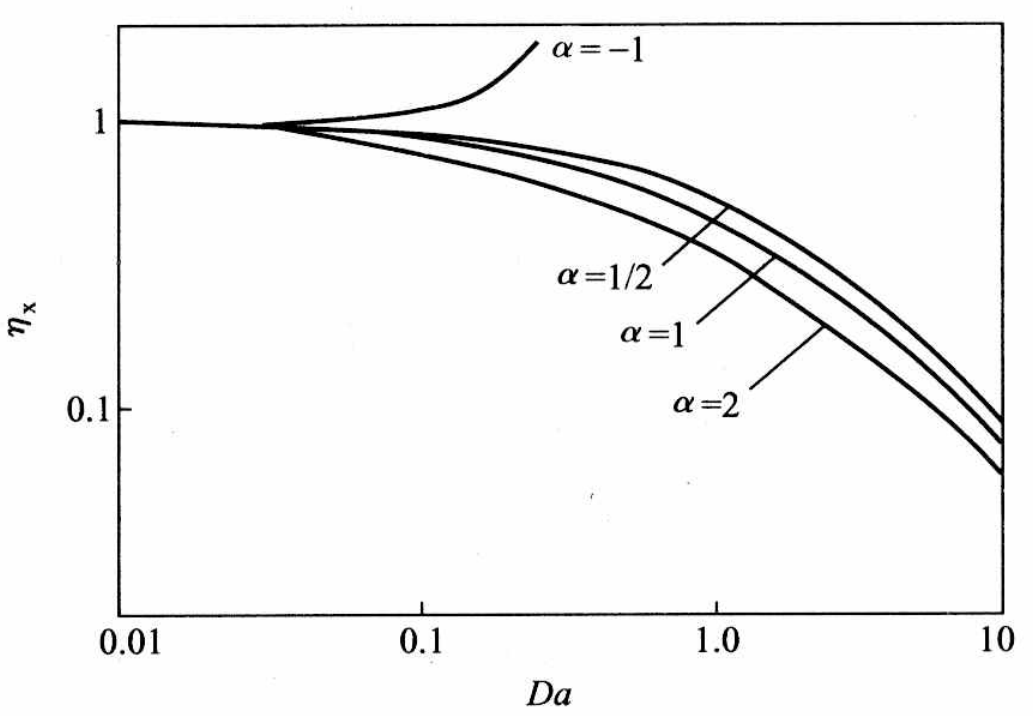
\includegraphics[width=\linewidth]{figures/fig6.2.png}
    \end{minipage}\hfill
    \begin{minipage}{0.4\linewidth}
        \begin{itemize}
            \item 除反应级数为负外，外扩散有效因子总是随丹克莱尔数的增加而降低；
            \item $\alpha$越大，外扩散有效因子随$Da$增加而下降得越明显；
            \item 无论$\alpha$为何值：$Da$趋于零时，$\eta_{\mathrm{X}}$总是趋于1。
        \end{itemize}
    \end{minipage}

    \bigskip
    反应级数越高，就越有必要采取措施降低外扩散阻力，以提高外扩散有效因子。

\end{frame}


\begin{frame}
    \frametitle{外扩散对多相催化反应的影响(平行反应)}

    考虑颗粒外表面与气相主体温度相同时的情况：
    \[
        \ch{A -> B} \qquad r_\mathrm{B} = k_1c_\mathrm{AS}^ \alpha
    \]
    \[
        \ch{A -> D} \qquad r_\mathrm{D} = k_2c_\mathrm{AS}^ \beta
    \]
    由反应瞬时选择性的定义可写出
    \[
        S = r_\mathrm{B}/(r_\mathrm{B} + r_\mathrm{D}) = 1/(1 + k_2 c_\mathrm{AS}^{\beta - \alpha}/k_1)
    \]
    如外扩散阻力甚小以致对过程无明显影响，则$c_\mathrm{AS} = c_\mathrm{AG}$，此时的瞬时选择性为
    \[
        S' = r_\mathrm{B}/(r_\mathrm{B} + r_\mathrm{D}) = 1/(1 + k_2 c_\mathrm{AG}^{\beta - \alpha}/k_1)
    \]

\end{frame}


\begin{frame}
    \frametitle{外扩散对多相催化反应的影响(平行反应)}

    比较以上二式可知，外扩散对于平行反应选择性的影响，取决于$\beta - \alpha$是正还是负
    \begin{itemize}
        \item 若$\alpha > \beta$，则$S < S'$
        
        外扩散影响的存在，使生成目的产物B的选择性降低，这是因为，外扩散阻力的存在，使得$c_\mathrm{AS} < c_\mathrm{AG}$，当生成目的产物B的反应级数大于副反应的反应级数时，外扩散阻力对主反应的影响程度大于对副反应的影响，故生成B的选择性下降；
        \item 若$\alpha < \beta$，则$S = S'$
        
        外扩散影响的存在，使生成目的产物B的选择性升高；
        \item 若$\alpha = \beta$，则$S = S'$
        
        外扩散不影响目的产物B的选择性。
    \end{itemize}

\end{frame}


\begin{frame}
    \frametitle{外扩散对多相催化反应的影响(连串反应)}

    对于一级不可逆连串反应
    \[
        \ce{A ->[k_1] B ->[k_2] D}
    \]
    B为目的产物，假设A、B和D的传质系数均相等，当过程为定态时可写出
    \[
        \begin{array}{l}
            k_{\mathrm{G}} a_{\mathrm{m}}\left(c_{\mathrm{AG}}-c_{\mathrm{AS}}\right)=k_{1} c_{\mathrm{AS}} \\
            k_{\mathrm{G}} a_{\mathrm{m}}\left(c_{\mathrm{BS}}-c_{\mathrm{BG}}\right)=k_{1} c_{\mathrm{AS}}-k_{2} c_{\mathrm{BS}} \\
            k_{\mathrm{G}} a_{\mathrm{m}}\left(c_{\mathrm{DS}}-c_{\mathrm{DG}}\right)=k_{2} c_{\mathrm{BS}}
            \end{array}
    \]
    由以上各式可得
    \[
        c_{\mathrm{AS}}=c_{\mathrm{AG}} /\left(1+D_{a 1}\right)
    \]
    \[
        c_{\mathrm{B}_{\mathrm{S}}}=\frac{D_{\mathrm{a} 1} c_{\mathrm{AG}}}{\left(1+D_{\mathrm{a} 1}\right)\left(1+D_{\mathrm{a} 2}\right)}+\left(\frac{c_{\mathrm{BG}}}{1+D_{\mathrm{a} 2}}\right)
    \]
    式中，$D_{\mathrm{a} 1}=k_{1} / k_{\mathrm{G}} a_{\mathrm{m}}, D_{\mathrm{a} 2}=k_{2} / k_{\mathrm{G}} a_{\mathrm{m}} $。

\end{frame}


\begin{frame}
    \frametitle{外扩散对多相催化反应的影响(连串反应)}

    反应的瞬时选择性
    \[
        S=\left(k_{1} c_{\mathrm{AS}}-k_{2} c_{\mathrm{BS}}\right) / k_{1} c_{\mathrm{AS}}=1-\frac{k_{2} D_{\mathrm{a} 1}}{k_{1}\left(1+D_{\mathrm{a} 2}\right)}-\frac{k_{2} c_{\mathrm{BG}}\left(1+D_{\mathrm{a} 1}\right)}{k_{1} c_{\mathrm{AG}}\left(1+D_{\mathrm{a} 2}\right)}
    \]
    由$D_{\mathrm{a} 1}$和$D_{\mathrm{a} 2}$的表达式可知
    \[
        D_{\mathrm{a} 2} = k_2 D_{\mathrm{a} 1}/k_1
    \]
    代入$S$表达式可得
    \[
        S=\frac{1}{1+D_{\mathrm{a} 2}}-\frac{k_{2} c_{\mathrm{BG}}\left(1+D_{\mathrm{a} 1}\right)}{k_{1} c_{\mathrm{AG}}\left(1+D_{\mathrm{a} 2}\right)} 
    \]
    当$D_{\mathrm{a} 1} = D_{\mathrm{a} 2} = 0$，即外扩散对过程没有影响时，上式变为
    \[
        S^{\prime}=1-k_{2} c_{\mathrm{BG}} / k_{1} c_{\mathrm{AG}}
    \]

\end{frame}


\begin{frame}
    \frametitle{外扩散对多相催化反应的影响(连串反应)}
    \[
        S^{\prime}=1-\frac{k_{2} c_{\mathrm{BG}}}{k_{1} c_{\mathrm{AG}}} 
    \]
    \[
        S=\frac{1}{1+D_{\mathrm{a} 2}}\left[ 1-\frac{k_{2} c_{\mathrm{BG}}\left(1+D_{\mathrm{a} 1}\right)}{k_{1} c_{\mathrm{AG}}} \right]
    \]
    外扩散阻力的存在，使连串反应的选择性降低，这是与平行反应不同之处。
    
    因此，对于连串反应，需设法降低外扩散阻力，以提高反应的选择性。
    
    例如萘氧化制苯酐、苯氧化制顺酐等氧化反应，需力求降低外扩散阻力，以避免深度氧化，从而增加目的产物的收率。

    若颗粒外表面与气相主体间，由于传热阻力而\bf{存在温度差}，如前所述，对于放热反应一般是$T_\mathrm{S} > T_\mathrm{G}$，这时，对复合反应选择性的影响决定于各反应的活化能。

\end{frame}


\begin{frame}[t]
    \frametitle{}

    \begin{example}
        \ce{A ->[k_1] B ->[k_2] D}为一级不可逆放热连串反应，已知$T_\mathrm{G} = \SI{450}{K}$，$c_\mathrm{BG}/c_\mathrm{AG} = 0.5$，$(T_\mathrm{S} - T_\mathrm{G}) = \SI{10}{K}$，$(k_\mathrm{G}a_\mathrm{m})_\mathrm{A} = (k_\mathrm{G}a_\mathrm{m})_\mathrm{B} = \SI{40}{cm^3/(g.s)}$，$k_1 = \num{6.0e8} \exp{[-E_1/RT]}$，\si{cm^3/(g.s)}，$k_2 = \num{1.2e6} \exp{[-E_2/RT]}$，\si{cm^3/(g.s)}，$E_1 = \SI{80.0}{kJ/mol}$，$E_2 = \SI{60.0}{kJ/mol}$。试求反应选择性。
    \end{example}
    \only<2>{
    \begin{itemize}
        \item[1.] 只考虑浓度差不考虑温度差
    \end{itemize}
        $T_\mathrm{S} = T_\mathrm{G} = \SI{450}{K}$

        $k_1 = \SI{0.310}{cm^3/(g.s)}$，$k_2 = \SI{0.130}{cm^3/(g.s)}$

        $D_\mathrm{a1} = 0.310/40 = \num{7.75e-3}$，$D_\mathrm{a2} = 0.130/40 = \num{3.25e-3}$

        考虑外扩散影响，$S = \frac{1}{1 + 3.25 \times 10^{-3}} - \frac{0.130(1 + 7.75 \times 10^{-3})0.5}{0.310(1 + 3.25 \times 10^{-3})} = 0.786$

        不考虑外扩散影响，$S' = 1 - 0.130 \times 0.5/0.310 = 0.790$
        }
        \only<3>{
            \begin{itemize}
                \item[2.] 同时考虑气相与颗粒外表面的浓度差与温度差
            \end{itemize}
            \[            
                T_\mathrm{S} =  \SI{460}{K},\qquad k_1 = \SI{0.494}{cm^3/(g.s)},\qquad  k_2 = \SI{0.184}{cm^3/(g.s)} 
            \]
            \[
                D_\mathrm{a1} = 0.01235,\qquad  D_\mathrm{a2} = 0.0046 
            \]
            \[
                S = \frac{1}{1 + 0.0046} - \frac{0.184(1.01235)0.5}{0.494(1.0046)} = 0.8077
            \]
        }
        \only<4>{
            
            \begin{itemize}
                \item[3.] 只考虑颗粒表面温度差，不考虑浓度差
            \end{itemize}
        不考虑外扩散影响，
        \[
            S'' = 1 - 0.184 \times 0.5/0.494 = 0.8138
        \]
        }
        

\end{frame}


\begin{frame}
    \frametitle{外扩散对多相催化反应的影响(连串反应)}

    \begin{itemize}
        \item $T_\mathrm{S} = T_\mathrm{G}$
        
        外扩散阻力的影响，总是使连串反应的选择性降低
        \item 放热反应，$T_\mathrm{S} > T_\mathrm{G}$
            \begin{itemize}
                \item[\bullet] 主反应活化能>副反应活化能
                
                选择性$S$比$S''$小，比$S'$大
                \item[\bullet] 主反应活化能<副反应活化能
            \end{itemize}
    \end{itemize}
\end{frame}


\begin{frame}[t]
    \frametitle{}

    \begin{example}
        在半径为R的球形催化剂上，等温进行气相反应\ch{A <=> B}。试以A或B的浓度为纵坐标，径向距离$r$为横坐标，针对下列三种情况分别绘出A和B的浓度分布示意图。
    
    （1）化学动力学控制

    （2）外扩散控制

    （3）内、外扩散的影响均不能忽略

    \end{example}

\end{frame}


\section{气体在多孔介质中的扩散}



\begin{frame}
    \frametitle{气体在多孔介质中的扩散}

        \begin{minipage}{0.48\linewidth}
            由于固体催化剂的多孔性，由颗粒内部孔道壁面所构成的内表面要比颗粒外表面大得多。所以，绝大多数反应物分子要沿着孔道向颗粒内部扩散，即所谓\highlight{内扩散}。
        \end{minipage}\hfill
        \begin{minipage}{0.48\linewidth}
            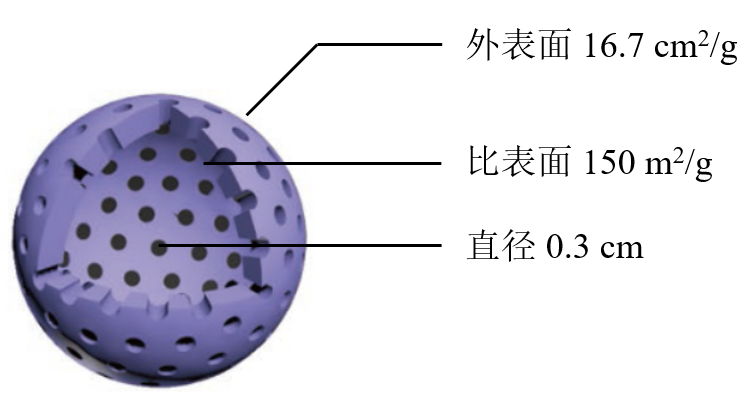
\includegraphics[width=\linewidth]{figures/surface.png}
        \end{minipage}

        与外扩散不同之处：
        \begin{enumerate}
          \item 内扩散是在孔道中进行，需要考虑气体分子与孔壁的碰撞。
          \item 内扩散是与反应并行进行的，反应物沿着孔道空间向粒内深处扩散的同时，就有反应物分子在孔壁面上发生催化反应。由于克服扩散阻力以及反应消耗，反应物的浓度逐渐下降，反应速率也相应地降低，到颗粒中心时反应物浓度最低（或等于零），反应速率也最小。
        \end{enumerate}

\end{frame}


\begin{frame}
    \frametitle{孔扩散}

    当孔内外不存在压力差，因而也就不存在由于压力差造成的层流流动时，流体中的某一组分靠扩散才可能进入孔内。因孔半径$r_\mathrm{a}$和分子运动平均自由程\footnote{气体分子相邻两次碰撞之间的平均距离}$\lambda$的相对大小的不同，孔扩散分为以下两种形式。
    \begin{itemize}
        \item 正常扩散 \qquad $\lambda /2r_\mathrm{a} \leqslant 10^{-2}$
        \item 努森扩散 \qquad $\lambda /2r_\mathrm{a} \geqslant 10$
    \end{itemize}
    当$\lambda /2r_\mathrm{a} \leqslant 10^{-2}$时，孔内扩散属正常扩散，这时的孔内扩散与通常的气体扩散完全相同。扩散速率主要受分子间相互碰撞的影响，与孔半径尺寸无关。对二组分气体A、B间的正常扩散系数$\mathscr{D}_\mathrm{AB}$，宜尽可能采用有关手册上的实验数据，缺乏实验数据时，或自己用实验测定，或用有关经验式估算。

\end{frame}


\begin{frame}
    \frametitle{二组分气体扩散系数}

    
二组分气体扩散系数可按下式估算
\[
    D_{\mathrm{AB}}=\frac{0.001 T^{1.75} \sqrt{\frac{1}{M_{\mathrm{A}}}+\frac{1}{M_{\mathrm{B}}}}}{p\left[(\Sigma V)_{\mathrm{A}}^{1 / 3}+(\Sigma V)_{\mathrm{A}}^{1 / 3}\right]^{2}}
\]
式中，$p$为总压，atm，$T$为绝对温度，K；$M_\mathrm{A}$和$M_\mathrm{B}$分别为A和B的相对分子质量；$(\Sigma V)_{\mathrm{A}}$和$(\Sigma V)_{\mathrm{B}}$分别为组分A及B的扩散体积。

由上式计算得到的扩散系数，单位为\si{cm^2/s}。由于该式为经验式，各有关数值的单位必须按规定使用。

一些简单原子和分子的扩散体积可以从物理化学手册中查取，对于手册中没有的一些复杂分子，其扩散体积可按照组成该分子的原子扩散体积进行加和得到。

\end{frame}


\begin{frame}
    \frametitle{多组分扩散}

    在化学反应过程中，经常遇到的是多组分扩散，在多组分流动物系中组分的扩散系数与物系组成有关，且各组分的扩散系数与扩散通量有一定的关系，此时组分A的扩散系数$D_\mathrm{1m}$可由下式计算
    \[
        \frac{1}{D_{1\mathrm{~m}}}=\sum_{j=2}^{n} \frac{y_{\mathrm{j}}-y_{1} N_{j} / N_{1}}{D_{1 j}} 
    \]
    上式称为Stefan-Maxwell方程。如果系统中无化学反应发生，系统中各组分扩散通量之比与其分子量之比存在如下关系
    \[
        N_{\mathrm{A}} / N_{\mathrm{B}}=\sqrt{M_{\mathrm{B}} / M_{\mathrm{A}}} 
    \]

\end{frame}


\begin{frame}
    \frametitle{多组分扩散}

    对于存在化学反应的系统，各组分的扩散通量与其化学计量系数成正比。存在化学反应的多组分系统中惰性组分I的扩散通量$N_1 = 0$。如果混合物系只有A$_1$组分扩散，其他组分均为不流动组分，则组分A$_1$向其余$n-1$个组分构成的混合物扩散，其扩散系数$D_\mathrm{1m}$可用下式计算
    \[
        \frac{1}{D_{1\mathrm{m}}}=\frac{1}{1-y_{1}} \sum_{j=2}^{n} \frac{y_{j}}{D_{1 j}}
    \]
    式中，$y_{j}$为组分A$_j$的摩尔分数；$D_\mathrm{1j}$为组分A$_1$与组分A$_j$所组成的二组分系统的扩散系数。

\end{frame}


\begin{frame}
    \frametitle{努森扩散系数}

    当$\lambda /2r_\mathrm{a} \geqslant 10$时，孔内扩散为努森扩散，这时主要是气体分子与孔壁的碰撞、而分子之间的相互碰撞则影响甚微，故分子在孔内的努森扩散系数$D_\mathrm{K}$只与孔半径$r_\mathrm{a}$有关，与系统中共存的其他气体无关。$D_\mathrm{K}$可按下式估算
    \[
        D_{\mathrm{K}}=9.7 \times 10^{3} r_{\mathrm{a}} \sqrt{T / M} 
    \]
    式中孔径$r_\mathrm{a}$的单位用cm，$D_\mathrm{K}$的单位为\si{cm^2/s}。
    
    不同压力下，气体分子的平均自由程入可用下式估算
    \[
        \lambda=1.013 / p \quad \mathrm{~cm}
    \]
    式中$p$的单位为Pa。

\end{frame}


\begin{frame}
    \frametitle{复合扩散系数}

    当气体分子的平均自由程与颗粒孔半径的关系介于上述两种情况之间时，$10^{-2} \leqslant \lambda /2r_\mathrm{a} \leqslant 10$，则两种扩散均起作用，这时应使用复合扩散系数$D$，对二组分扩散有
    \[
        D_{\mathrm{A}}=\frac{1}{1 /(D_{\mathrm{K}})_{\mathrm{A}}+(1-b y_{\mathrm{A}}) / D_{\mathrm{AB}}}
    \]
    \vspace{-10 pt}    
    \[
        b=1+N_{\mathrm{B}} / N_{\mathrm{A}}
    \]
    式中，$N_{\mathrm{A}}$、$N_{\mathrm{B}}$为气体A和B的扩散通量，$y_{\mathrm{A}}$为气体A的摩尔分数，$D_{\mathrm{A}}$为A气体的复合扩散系数，$(D_{\mathrm{K}})_{\mathrm{A}}$为气体A的努森扩散系数。上式中含有$b$与$y_{\mathrm{A}}$，而$b$又与$N_{\mathrm{A}}$、$N_{\mathrm{B}}$有关，使用起来不方便。
    
    若为等摩尔二组分逆向扩散，则$N_{\mathrm{A}} = -N_{\mathrm{B}}$，上式可简化为
    \[
        D_{\mathrm{A}}=\frac{1}{1 /(D_{\mathrm{K}})_{\mathrm{A}}+1 / {D}_{\mathrm{AB}}}
    \]

\end{frame}


\begin{frame}
    \frametitle{有效扩散系数}

    上面讨论的是单一孔道中的扩散，在多孔催化剂或多孔固体颗粒中，组分$i$的摩尔扩散通量为
    \[
        N_{i}=-\frac{P}{R T} D_{\mathrm{e} i} \frac{\mathrm{d} y_{i}}{\mathrm{~d} Z}=-D_{\mathrm{e} i} \frac{\mathrm{d} c_{i}}{\mathrm{~d} Z} 
    \]
    式中$D_{\mathrm{e} i}$为组分$i$在催化剂中的有效扩散系数，$Z$为气体组分$i$的扩散距离。当催化剂粒内孔道是任意取向，而颗粒的孔隙率为$\varepsilon_{\mathrm{p}}$时，对颗粒的单位外表面而言，微孔开口所占的分率也是$\varepsilon_{\mathrm{p}}$。孔道间会有相互交叉，各孔道的形状和每根孔道的不同部位的截面积也会有差异，由于这些因素，使得在颗粒中的扩散距离与在圆柱形孔道中的扩散距离有所不同，通常是引入一校正参数$\tau_{\mathrm{m}}$，称为曲节因子，其数值因催化剂颗粒的孔结构而变化，范围多在3～5之间。校正后的扩散距离为$\tau_{\mathrm{m}}Z$，由上可得催化剂颗粒的有效扩散系数为
    \[
        D_{\mathrm{e} i}=\varepsilon_{\mathrm{p}} D_{i} / \tau_{\mathrm{m}}
    \]

\end{frame}


\begin{frame}[t]
    \frametitle{}

    \begin{example}
        噻吩(\ch{C4H4S})在氢气中于600K、\SI{3.04}{MPa}时，在催化剂颗粒中进行扩散。用BET法测得催化剂的比表面为\SI{180}{m^2/g}，孔隙率为0.4，颗粒密度为\SI{1.4}{g/cm^3}，而且测知其孔径分布相当集中，试计算噻吩在上述条件下于该催化剂中的有效扩散系数。巳知$\tau_{\mathrm{m}} = 3.0$，噻吩与氢二组分分子扩散系数等于\SI{0.0457}{cm^2/s}。
    \end{example}\pause
    $\begin{aligned}
        V_{\mathrm{g}} &=\varepsilon_{\mathrm{p}} / \rho_{\mathrm{p}} \\
        \left\langle r_{\mathrm{a}}\right\rangle &= 2V_{\mathrm{g}}/S_{\mathrm{g}} = 2 \varepsilon_{\mathrm{p}} / S_{\mathrm{g}} \rho_{\mathrm{p}}=2 \times 0.4 /(180 \times 1.4 \times 10^{4})=31.7 \times 10^{-8} \mathrm{~cm} \\
        (D_{\mathrm{K}})_{\mathrm{A}} &=9.7 \times 10^{3} \times 31.7 \times 10^{-8} \sqrt{600 / 84}=8.22 \times 10^{-3} \mathrm{~cm}^{2} / \mathrm{s} \\
        D_{\mathrm{A}} &=\frac{1}{1 /(D_{\mathrm{K}})_{\mathrm{A}}+1 / \mathscr{D}_{\mathrm{AB}}}=\frac{1}{1000 / 8.22+1 / 0.0454}=6.97 \times 10^{-3} \mathrm{~cm}^{2} / \mathrm{s} \\
        D_{\mathrm{eA}} &= \varepsilon_{\mathrm{p}} D_{\mathrm{A}}/ \tau_{\mathrm{m}}=6.97 \times 10^{-3} \times 0.4 / 3=9.29 \times 10^{-4} \mathrm{~cm}^{2} / \mathrm{s}
        \end{aligned}$

\end{frame}


\section{多孔催化剂中的扩散与反应}


\begin{frame}
    \frametitle{多孔催化剂中的扩散与反应}

        \begin{minipage}{0.48\linewidth}
            外扩散时反应物要先扩散到颗粒外表面才可发生反应，而内扩散是与反应并行进行的，即反应物沿着孔道空间向粒内深处扩散的同时，就有反应物分子在孔壁面上发生催化反应。
        \end{minipage}\hfill
        \begin{minipage}{0.48\linewidth}
            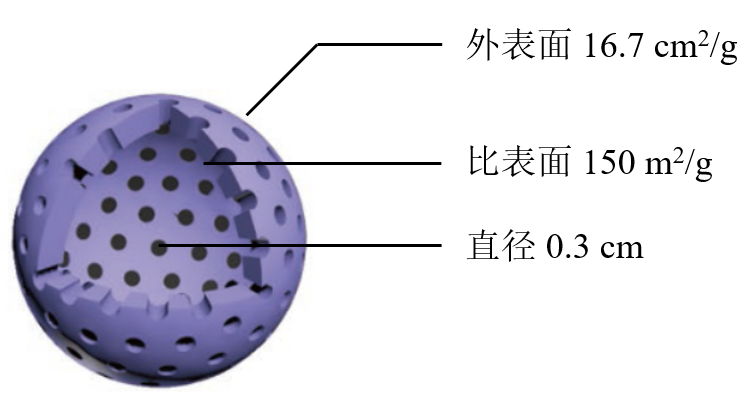
\includegraphics[width=\linewidth]{figures/surface.png}
        \end{minipage}

        \begin{itemize}
          \item 如果反应速率较慢，而反应组分的有效扩散系数又较大，则孔道内外只需很小的浓度差，便能供给孔内表面反应所消耗的反应物，孔壁各处所接触的反应物浓度几乎都等于孔口处的浓度，通常认为这时整个颗粒的内表面都得到了充分的利用。
          \item 若反应速率相当快，反应物进入孔道内不长的距离即已反应完全，这时颗粒内表面没有得到充分的利用。
        \end{itemize}

\end{frame}


\begin{frame}
    \frametitle{多孔催化剂内反应组分的浓度分布}
    多孔催化剂内反应组分的浓度分布是不均匀的，温度一定时，浓度的高低直接影响反应速率的大小。所以，确定催化剂颗粒内反应组分的浓度分布就十分必要。

        \begin{minipage}{0.65\linewidth}
            考察如图所示的薄片催化剂，在其上进行一级不可逆反应。设该催化剂颗粒是等温的，且其孔隙结构均匀，各向同性。为了确定颗粒内反应物A的浓度分布，需先建立描述此过程的反应---扩散微分方程。为此，可在颗粒内取一厚度为$\dif Z$的微元，对此微元作反应物A的物料衡算即可。

            \bigskip
            
            \quad 单位时间内扩散进入微元的组分A量

            $-$单位时间内由微元扩散出的组分A量

            $=$在微元内反应掉的组分A量
        \end{minipage}\hfill
        \begin{minipage}{0.32\linewidth}
            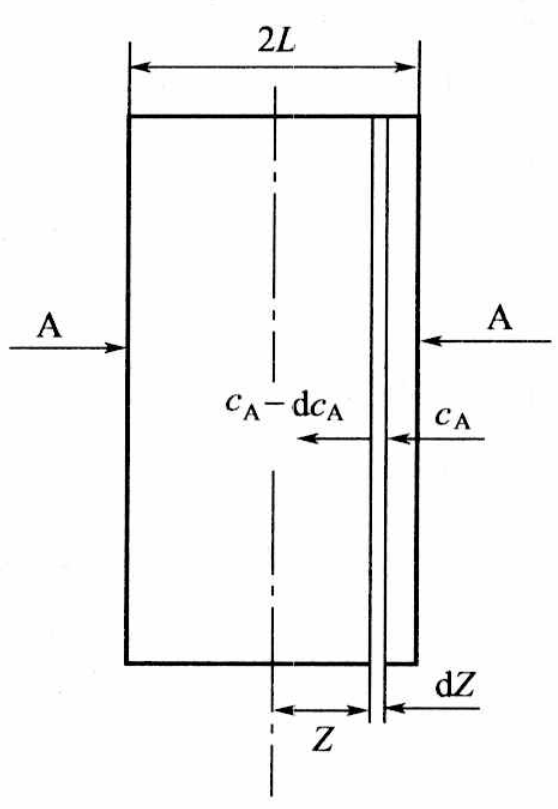
\includegraphics[width=\linewidth]{figures/fig6.3.png}
        \end{minipage}

\end{frame}


\begin{frame}
    \frametitle{多孔催化剂内反应组分的浓度分布}

        \begin{minipage}{0.65\linewidth}
            设有效扩散系数$D_\mathrm{e}$为常数，扩散面积为$a$，则
            \[
                D_{\mathrm{e}} a\left(\frac{\mathrm{d} c_{\mathrm{A}}}{\mathrm{d} Z}\right)_{\mathrm{Z}+\mathrm{d} Z}-D_{\mathrm{e}} a\left(\frac{\mathrm{d} c_{\mathrm{A}}}{\mathrm{d} Z}\right)_{\mathrm{Z}}=k_{\mathrm{p}} c_{\mathrm{A}} a \mathrm{~d} Z
            \]
            $k_\mathrm{p}$系以催化剂颗粒体积为基准的反应速率常数。
            \[
                \left(\frac{\mathrm{d} c_{\mathrm{A}}}{\mathrm{d} Z}\right)_{\mathrm{Z}+\mathrm{d} Z}=\left(\frac{\mathrm{d} c_{\mathrm{A}}}{\mathrm{d} Z}\right)_{\mathrm{Z}}+\frac{\mathrm{d}}{\mathrm{d} Z}\left(\frac{\mathrm{d} c_{\mathrm{A}}}{\mathrm{d} Z}\right) \mathrm{d} Z
            \]
            代入化简后得
            \[
                \frac{\mathrm{d}^{2} c_{\mathrm{A}}}{\mathrm{d} Z^{2}}=\frac{k_{\mathrm{p}}}{D_{\mathrm{e}}} c_{\mathrm{A}}
            \]
            这就是薄片催化剂上进行一级不可逆反应时的反应扩散方程。（二阶微分方程）
        \end{minipage}\hfill
        \begin{minipage}{0.32\linewidth}
            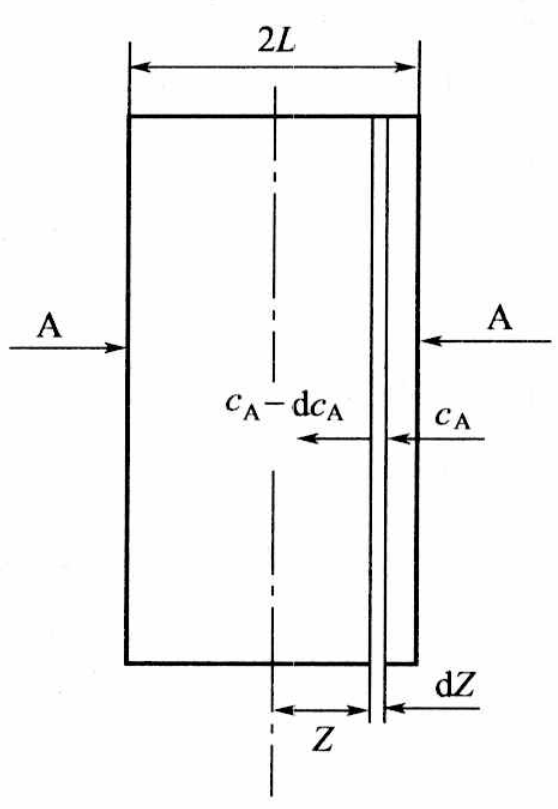
\includegraphics[width=\linewidth]{figures/fig6.3.png}
        \end{minipage}

\end{frame}


\begin{frame}
    \frametitle{多孔催化剂内反应组分的浓度分布}

    $\frac{\mathrm{d}^{2} c_{\mathrm{A}}}{\mathrm{d} Z^{2}}=\frac{k_{\mathrm{p}}}{D_{\mathrm{e}}} c_{\mathrm{A}}$，结合其边界条件 $\begin{cases}
        Z=L, c_{\mathrm{A}}=c_{\mathrm{AS}} \\
    
        Z=0, \mathrm{~d} c_{\mathrm{A}} / \mathrm{d} Z=0    
    \end{cases}$

    解之得催化剂颗粒内反应物的浓度分布。

    引入下列无量纲量
    \[
        \xi=c_{\mathrm{A}} / c_{\mathrm{AS}}, \quad \zeta=Z / L, \quad \phi^{2}=L^{2} \frac{k_{p}}{D_{\mathrm{e}}}
    \]
    无量纲化得
    \[
        \frac{\mathrm{d}^{2} \xi}{\mathrm{d} \zeta^{2}}=\phi^{2} \xi
    \]
    \[
        \zeta=1 \qquad \qquad \xi=1
    \]
    \[
        \zeta=0 \quad \mathrm{~d} \xi / \mathrm{d} \zeta=0
    \]

\end{frame}


\begin{frame}
    \frametitle{多孔催化剂内反应组分的浓度分布}

    上式为二阶常系数线性齐次微分方程，其通解为
    \[
        \xi=A \mathrm{e}^{\phi \zeta}+B \mathrm{e}^{-\phi \zeta}
    \]
    结合边界条件，可求得积分常数A及B为
    \[
        \mathrm{A}=\mathrm{B}=1 /(\mathrm{e}^{\phi}+\mathrm{e}^{-\phi})
    \]
    代回，得
    \[
        \xi=\frac{\mathrm{e}^{\phi \zeta}+\mathrm{e}^{-\phi \zeta}}{\mathrm{e}^{\phi}+\mathrm{e}^{-\phi}}=\frac{\cosh (\phi \zeta)}{\cosh (\phi)}
    \]
    或
    \[
        \frac{c_{\mathrm{A}}}{c_{\mathrm{AS}}}=\frac{\cosh (\phi Z / L)}{\cosh (\phi)}
    \]
    这便是薄片催化剂内反应物的浓度分布方程。

\end{frame}


\begin{frame}
    \frametitle{多孔催化剂内反应组分的浓度分布}

        \begin{minipage}{0.55\linewidth}
            为了直观地考察其变化规律，以$\phi $为参数，以$\xi$对$\zeta$作图，如图所示。
            \begin{itemize}
                \item 无论$\phi $为何值，无量纲浓度$\xi$总是随无量纲距离$\zeta$的减小而降低，即从颗粒外表面到颗粒中心处反应物A的浓度逐渐降低。
                \item $\phi $值不同，其降低的程度也不同：$\phi $值越大，反应物的浓度变化越急剧。
            \end{itemize}
        \end{minipage}\hfill
        \begin{minipage}{0.4\linewidth}
            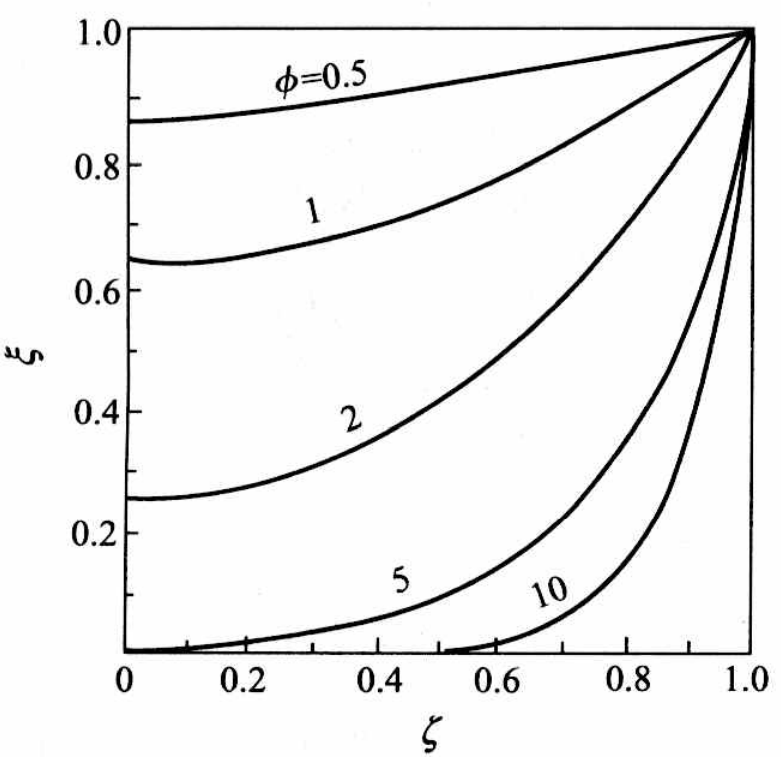
\includegraphics[width=\linewidth]{figures/fig6.4.png}
        \end{minipage}

        颗粒内的浓度分布是反应物的扩散与反应综合作用的结果，而$\phi $值的大小又反映了浓度分布的特征，从$\phi $值可以判断内扩散对反应过程的影响程度。

\end{frame}


\begin{frame}
    \frametitle{梯尔模数}

    无量纲参数$\phi$叫做梯尔(Thiele)模数，是处理扩散与反应问题的一个极其重要的特征参数。
    
    根据前面对梯尔模数所下的定义，作适当的改写可得其物理意义为
    \[
        \phi^{2}=L^{2} \frac{k_{\mathrm{p}}}{D_{\mathrm{e}}}=\frac{a L k_{\mathrm{p}} c_{\mathrm{AS}}}{D_{\mathrm{e}} a(c_{\mathrm{AS}}-0) / L}=\frac{\text { 表面反应速率 }}{\text { 内扩散速率 }} 
    \]
    由此可知梯尔模数表示表面反应速率与内扩散速率的相对大小。
    \begin{itemize}
        \item $\phi$值越大，表明表面反应速率大而内扩散速率小，
        
        说明内扩散阻力对反应过程的影响大。
        \item $\phi$值越小，说明内扩散阻力对反应过程的影响越小。
    \end{itemize}
    
\end{frame}


\begin{frame}
    \frametitle{薄片催化剂的内扩散有效因子}

    为了计算催化剂颗粒上的反应速率，引用内扩散有效因子$\eta$，其定义如下
    \[
        \eta=\frac{\text { 内扩散对过程有影响时的反应速率 }}{\text { 内扩散对过程无影响时的反应速率 }} 
    \]
    内扩散有影响时催化剂颗粒内的浓度是不均匀的，需求出此时的平均反应速率
    \[
        \left\langle r_{\mathrm{A}}\right\rangle=\frac{1}{L} \int_{0}^{L} k_{\mathrm{p}} c_{\mathrm{A}} \mathrm{d} Z
    \]
    将$\frac{c_{\mathrm{A}}}{c_{\mathrm{A}_{\mathrm{S}}}}=\frac{\cosh (\phi Z / L)}{\cosh (\phi)}$代入，得
    \[
        \left\langle r_{\mathrm{A}}\right\rangle=\frac{k_{\mathrm{p}} c_{\mathrm{AS}}}{L \cos h \phi} \int_{0}^{L} \cosh (\phi Z / L) \mathrm{d} Z=\frac{k_{\mathrm{p}} c_{\mathrm{AS}} \tan h(\phi)}{\phi}
    \]
    这即为内扩散有影响时的反应速率。

\end{frame}


\begin{frame}
    \frametitle{薄片催化剂的内扩散有效因子}

    内扩散没有影响时，颗粒内部处的浓度均与外表面上的浓度$c_{\mathrm{AS}}$相等，因之，相应的反应速率为$k_{\mathrm{p}}c_{\mathrm{AS}}$，把这两个反应速率代入内扩散有效因子定义式，化简后可得
    \[
        \eta=\tanh (\phi) / \phi 
    \]
    这便是在薄片催化剂上进行一级不可逆反应时，内扩散有效因子的计算公式。
    \begin{minipage}{0.52\linewidth}
        \only<1>{
            \begin{itemize}
            \item $\eta$值总是随$\phi$值的增大而单调地下降
            \item $\phi$值越大，内扩散的影响也越大
        \end{itemize} 
        \begin{redblock}{思考}
            如何减小$\phi$值以降低内扩散的影响？
        \end{redblock}
        }
        \only<2>{
           \begin{itemize}
            \item $\eta$值总是随$\phi$值的增大而单调地下降
            \item $\phi$值越大，内扩散的影响也越大
            \item 减小催化剂颗粒的尺寸，$\phi$值减小
            \item 增大催化剂的孔容和孔半径，可提高有效扩散系数$D_\mathrm{e}$的值，从而使$\phi$值减小
        \end{itemize} 
        }
    \end{minipage}\hfill
    \begin{minipage}{0.44\linewidth}
        \begin{figure}[htpb]
            \centering
            
\includegraphics[width=.8\linewidth]{薄片}
        \end{figure}
    \end{minipage}
\end{frame}


\begin{frame}
    \frametitle{内扩散有效因子的推导}

    内扩散有效因子计算式的推导可概括为如下几步：
    \begin{enumerate}
        \item 建立催化剂颗粒内反应物浓度分布的微分方程，即扩散反应方程，确定相应的边界条件；解此微分方程而求得浓度分布；
        \item 根据浓度分布而求得颗粒内的平均反应速率；
        \item 由内扩散有效因子的定义即可导出其计算式。
    \end{enumerate}

    按此步骤可导出其他几何形状的催化剂颗粒的内扩散有效因子计算式。

\end{frame}


\begin{frame}
    \frametitle{球形催化剂颗粒的内扩散有效因子}

    对于半径为$R_\mathrm{p}$的球形催化剂粒子，在粒内进行等温一级不可逆反应，取任一半径$r$处厚度为$\dif r$的壳层，对组分A作物料衡算。其扩散反应方程为
        \begin{minipage}{0.55\linewidth}
            \[
                \frac{\mathrm{d}^{2} c_{\mathrm{A}}}{\mathrm{d} r^{2}}+\frac{2}{r} \frac{\mathrm{d} c_{\mathrm{A}}}{\mathrm{d} r}=\frac{k_{\mathrm{p}}}{D_{\mathrm{e}}} c_{\mathrm{A}}
            \]
            对于半径为$R_\mathrm{p}$的无限长圆柱或两端面无孔的有限长圆柱，其扩散反应方程为
            \[
                \frac{\mathrm{d}^{2} c_{\mathrm{A}}}{\mathrm{d} r^{2}}+\frac{1}{r} \frac{\mathrm{d} c_{\mathrm{A}}}{\mathrm{d} r}=\frac{k_{\mathrm{p}}}{D_{\mathrm{e}}} c_{\mathrm{A}}
            \]            
        \end{minipage}\hfill
        \begin{minipage}{0.42\linewidth}
            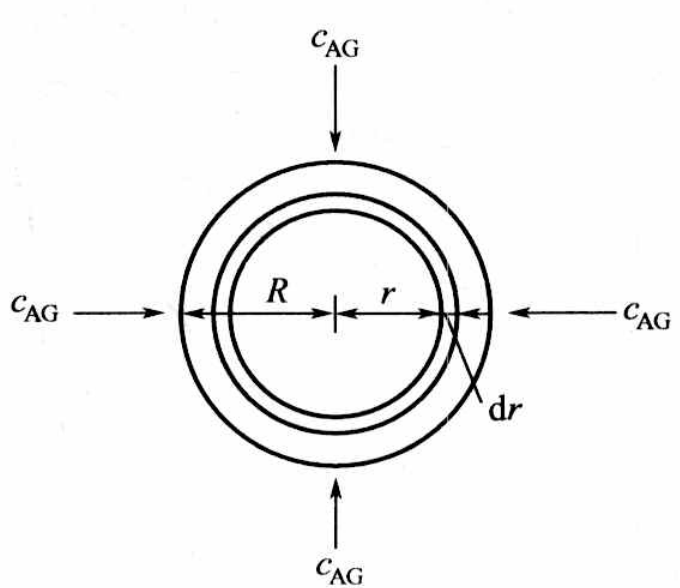
\includegraphics[width=\linewidth]{figures/fig6.6.png}
        \end{minipage}

\end{frame}


\begin{frame}
    \frametitle{圆球圆柱催化剂颗粒的内扩散有效因子}

    无论球形还是圆柱，都可采用下列边界条件
    \[
        r=R_{\mathrm{p}}, \quad c_{\mathrm{A}}=c_{\mathrm{AS}}
    \]
    \[
        r=0, \quad \mathrm{~d} c_{\mathrm{A}} / \mathrm{d} r=0
    \]
    结合给定的边界条件，这两个方程的解分别为
    \[
        \text{圆球：} \qquad \frac{c_{\mathrm{A}}}{c_{\mathrm{AS}}}=\frac{R_{\mathrm{p}} \sin h\left(3 \phi r / R_{\mathrm{p}}\right)}{r \sin h(3 \phi)}
    \]
    \[
        \text{圆柱：} \qquad \frac{c_{\mathrm{A}}}{c_{\mathrm{AS}}}=\frac{I_{0}\left(2 \phi r / R_{\mathrm{p}}\right)}{I_{0}(2 \phi)} \qquad ~
    \]
    式中$I_{0}$为零阶一类变型贝塞尔函数。

\end{frame}


\begin{frame}
    \frametitle{圆球圆柱催化剂颗粒的内扩散有效因子}

    式中$\phi$为适用于不同几何形状的催化剂颗粒的梯尔模数
    \[
        \phi=\frac{V_{\mathrm{p}}}{a_{\mathrm{p}}} \sqrt{\frac{k_{\mathrm{p}}}{D_{\mathrm{e}}}}
    \]
    其中$V_{\mathrm{p}}$和$a_{\mathrm{p}}$分别为颗粒的体积与外表面积，此式与前面对薄片催化剂而定义的梯尔模数完全一致。

    根据浓度分布式分别求出粒内平均反应速率，再用定义式即可导出圆球及圆柱的内扩散有效因子计算式如下：
    \[
        \text{圆球：} \qquad \eta =\frac{1}{\phi}\left[\frac{1}{\tan h(3 \phi)}-\frac{1}{3 \phi}\right]
    \]
    \[
        \text{圆柱：} \qquad \eta =I_{1}(2 \phi) /\left[\phi I_{0}(2 \phi)\right] \quad
    \]
    式中$I_{1}$为一阶一类变型贝塞尔函数，其值可从贝塞尔函数表中查得。

\end{frame}


\begin{frame}
    \frametitle{不同几何形状的催化剂颗粒的内扩散有效因子}
        \begin{minipage}{0.55\linewidth}
            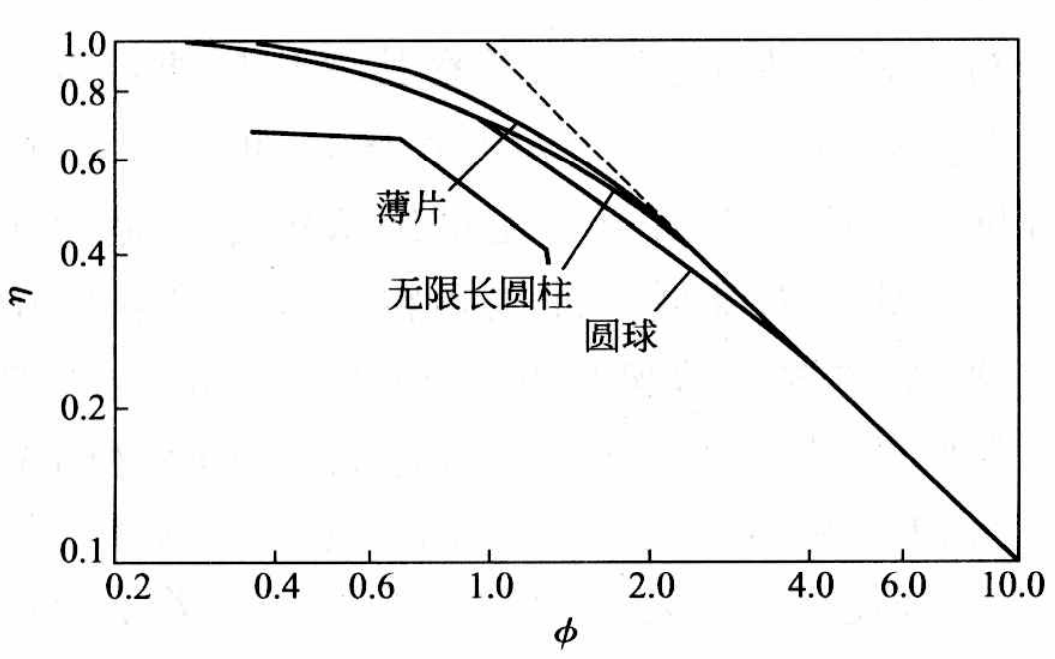
\includegraphics[width=\linewidth]{figures/fig6.5.png}
        \end{minipage}\hfill
        \begin{minipage}{0.4\linewidth}
            比较不同几何形状的催化剂颗粒的内扩散有效因子，图上三条曲线几乎重合为一，特别是值较小或值较大时更为明显。
        \end{minipage}
        
        只有当$0.4 < \phi <3$时，三者才有较明显的差别。纵使在这一区域内，它们之间相差只不过$10\% \sim 20\%$。
    
    所以，对任何几何形状的催化剂颗粒，均可按前述$\eta$计算式计算得到可接受的内扩散有效因子值。
            
\end{frame}


\begin{frame}
    \frametitle{内扩散有效因子}

    无论是何种形状的催化剂颗粒，
    \begin{itemize}
        \item 当$\phi<0.4$时，$\eta \approx 1$，即内扩散的影响可忽略。
        \item 当$\phi>3.0$时，即内扩散影响严重时，三条曲线与其渐近线（图中的虚线）
        相重合，此时$$\eta = 1/\phi$$

        在此情况下，对于任何形状的催化剂颗粒，都可用此式来估算内扩散有效因子。
    \end{itemize}

    最后需要再次指出，\bf{以上的讨论只适用于等温下进行一级不可逆反应的情况}。

\end{frame}


\begin{frame}[t]
    \frametitle{}
    \begin{example}
        乙烯直接水合制乙醇的初始反应速率符合一级反应动力学方程。在300℃，7.0 MPa时，其反应速率常数为0.09 s$^{-1}$。催化剂颗粒直径为5 mm，有效扩散系数$D_\mathrm{e} = 7.04\times 10^{-4}$ \si{cm^2/s}。试求催化剂颗粒的内部效率因子。
        \tcblower
        \pause
        $\phi = \frac{d}{6}\sqrt{\frac{k_\mathrm{p}}{D_\mathrm{eA}}} = \frac{0.5}{6}\sqrt{\frac{0.09}{7.04\times 10^{-4}}} = 0.94$

$\eta = \frac{1}{\phi}[\frac{1}{\mathrm{tan}h (3\phi)}-\frac{1}{3\phi}] = \frac{1}{0.94}[\frac{1}{\tanh (3\times 0.94)}-\frac{1}{3\times 0.94}] = 0.694$
    \end{example}
\end{frame}


\begin{frame}[t]
    \frametitle{}

    \begin{block}{例6.5}
        在铬铝催化剂上进行丁烷脱氢反应，其反应速率方程为
        \[
            r_{\mathrm{A}} =k_{\mathrm{W}} c_{\mathrm{A}} \quad \mathrm{mol} /(\mathrm{g} \cdot \mathrm{s})
        \]
        0.1013 MPa及773 K时，$k_\mathrm{W} = \SI{0.92}{cm^3/(g.s)}$。若在该温度下采用厚度为8 mm的薄片催化剂进行反应，催化剂平均孔半径为\SI{48e-10}{m}，孔容为\SI{0.35}{cm^3/g}，曲节因子等于2.5。试计算内扩散有效因子。
    \tcblower
    \only<2>{
        \vspace{-1pt}
    $\begin{aligned}
        \frac{\lambda}{2 r_{\mathrm{a}}} &=\frac{10^{-5}}{2 \times 48 \times 10^{-8}}=10.4>10 \\
        D_{\mathrm{K}} &=9700\left(48 \times 10^{-8}\right)(773 / 58)^{1 / 2}=1.70 \times 10^{-2} \mathrm{~cm}^{2} / \mathrm{s} \\
        D_{\mathrm{eA}} &=V_{\mathrm{g}} \rho_{\mathrm{p}} D_{\mathrm{K}} / \tau_{\mathrm{m}}=0.35\left(1.70 \times 10^{-2}\right) \rho_{\mathrm{p}} / 2.5=2.38 \times 10^{-3} \rho_{\mathrm{p}} \quad \mathrm{cm}^{2} / \mathrm{s} \\
        k_{\mathrm{p}} &=k_{\mathrm{W}} \rho_{\mathrm{p}}=0.92 \rho_{\mathrm{p}} \quad \mathrm{s}^{-1}
        \end{aligned}$
        }
        \only<3>{
            $\begin{aligned}        
                \phi &=\frac{0.8}{2}\sqrt{\frac{0.92 \rho_{\mathrm{p}}}{2.38 \times 10^{-3} \rho_{\mathrm{p}}}}=7.86 \\
                \eta &= \tanh (7.86)/7.86 = 0.127
            \end{aligned}$
        
            由于$\phi = 7.86>3$，内扩散影响相当严重，用简化式计算$\eta$所得的值与用精确式计算完全一致。
            }
    \end{block}
\end{frame}



\begin{frame}[t]
    \frametitle{}

    \begin{example}
        在等温球形催化剂上进行一级可逆反应\ch{A <=> B}，试推导内扩散有效因子计算式。
    \end{example}

\end{frame}


\begin{frame}
    \frametitle{非一级反应的内扩散有效因子}

    处理非一级反应的扩散反应问题，原则上，前面所采用的方法与步骤完全适用，只是在数学处理上比较繁琐。

    设在等温薄片催化剂上进行某一化学反应，其速率方程为
    \[
        r_{\mathrm{A}}=k_{\mathrm{p}} f(c_{\mathrm{A}})
    \]
    设有效扩散系数$D_\mathrm{e}$为常数，扩散反应方程为
    \[
        \frac{\mathrm{d}^{2} c_{\mathrm{A}}}{\mathrm{d} Z^{2}}=\frac{k_{\mathrm{p}}}{D_{\mathrm{e}}} f(c_{\mathrm{A}})
    \]
    \[
        \text{因} \quad \frac{\mathrm{d}^{2} c_{\mathrm{A}}}{\mathrm{d} Z^{2}}=\frac{\mathrm{d} c_{\mathrm{A}}}{\mathrm{d} Z}\left[\frac{\mathrm{d}}{\mathrm{d} c_{\mathrm{A}}} \times \frac{\mathrm{d} c_{\mathrm{A}}}{\mathrm{d} Z}\right] \quad \text{并设} \quad p = \dif c_\mathrm{A}/\dif Z \quad \text{则}
    \]
    \[
        p \frac{\mathrm{d} p}{\mathrm{~d} c_{\mathrm{A}}}=\frac{k_{\mathrm{p}}}{D_{\mathrm{e}}} f(c_{\mathrm{A}})
    \]

\end{frame}


\begin{frame}
    \frametitle{非一级反应的内扩散有效因子}

    \[
        z=L \quad c_{\mathrm{A}}=c_{\mathrm{AS}} \quad p=p_{\mathrm{S}}=(\mathrm{d} c_{\mathrm{A}} / \mathrm{d} Z)_{\mathrm{S}}
    \]
    \[
        z=0 \quad c_{\mathrm{A}}=c_{\mathrm{AC}}=\dif c_{\mathrm{A}} / \mathrm{d} Z=0 \qquad \quad
    \]
    积分$p \frac{\mathrm{d} p}{\mathrm{~d} c_{\mathrm{A}}}=\frac{k_{\mathrm{p}}}{D_{\mathrm{e}}} f(c_{\mathrm{A}})$得
    \[
        p_{\mathrm{S}}=\left(\frac{\mathrm{d} c_{\mathrm{A}}}{\mathrm{d} Z}\right)_{\mathrm{S}}=\left[\frac{2 k_{\mathrm{p}}}{D_{\mathrm{e}}} \int_{c_{\mathrm{AC}}}^{c_{\mathrm{AS}}} f(c_{\mathrm{A}}) \mathrm{d} c_{\mathrm{A}}\right]^{1 / 2}
    \]
    扩散进入催化剂颗粒的组分A量为
    \[
        D_{\mathrm{e}} a_{\mathrm{p}}\left(\frac{\mathrm{d} c_{\mathrm{A}}}{\mathrm{d} Z}\right)_{\mathrm{S}}=D_{\mathrm{e}} a_{\mathrm{p}}\left[\frac{2 k_{\mathrm{p}}}{D_{\mathrm{e}}} \int_{c_{\mathrm{AC}}}^{c_{\mathrm{AS}}} f(c_{\mathrm{A}}) \mathrm{d} c_{\mathrm{A}}\right]^{1 / 2}
    \]
    对于定态过程，这也等于在颗粒内起反应的组分A量。

\end{frame}


\begin{frame}
    \frametitle{非一级反应的内扩散有效因子}

    如果内扩散没有影响，则催化剂颗粒内组分A的浓度与外表面处的浓度$c_{\mathrm{AS}}$相等，相应起反应的组分A量应为$La_\mathrm{p}k_\mathrm{p}f(c_{\mathrm{AS}})$。将这两个量代入定义式整理后可得内扩散有效因子为
    \[
        \eta=\frac{\sqrt{2 D_{\mathrm{e}}}}{L \sqrt{k_{\mathrm{p}}} f(c_{\mathrm{AS}})}\left[\int_{c_{\mathrm{AC}}}^{c_{\mathrm{AS}}} f(c_{\mathrm{A}}) \mathrm{d} c_{\mathrm{A}}\right]^{1 / 2}
    \]
    用此式来计算最大的困难是催化剂中心浓度未知，也难以用实验测定。
    
    当内扩散影响大时，对于不可逆反应，颗粒中心浓度$c_{\mathrm{AC}} \approx 0$；
    
    对于可逆反应，则$c_{\mathrm{AC}} \approx  c_{\mathrm{Ae}}$，而$c_{\mathrm{Ae}}$是可以计算出来的。
    \[
        \eta=\frac{a_{\mathrm{p}} \sqrt{2 D_{\mathrm{e}}}}{V_{\mathrm{p}} \sqrt{k_{\mathrm{p}}} f(c_{\mathrm{AS}})}\left[\int_{c_{\mathrm{AC}}}^{c_{\mathrm{AS}}} f(c_{\mathrm{A}}) \mathrm{d} c_{\mathrm{A}}\right]^{1 / 2}
    \]
    此式可用于其他几何形状的催化剂颗粒。

\end{frame}


\begin{frame}
    \frametitle{内外扩散都有影响时的有效因子}

    若反应过程中内、外扩散都有影响，则定义总有效因子为
    \[
        \eta_0 = \frac{\text{内外扩散都有影响时的反应速率}}{\text{无扩散影响时的反应速率}}
    \]
    对一级反应可以写出
    \[
        (-\mathscr{R}_{\mathrm{A}})=k_{\mathrm{G}} a_{\mathrm{m}}(c_{\mathrm{AG}}-c_{\mathrm{AS}})=\eta k_{\mathrm{W}} c_{\mathrm{AS}}=\eta_{0} k_{\mathrm{W}} c_{\mathrm{AG}}
    \]
    在反应过程达到定态时这三个等式是等效的，第一式表示反应速率与外扩散速率相等；第二式是以内扩散有效因子表示的反应速率，式中的$c_{\mathrm{AS}}$已暗含着外扩散的影响；第三式是以总有效因子表示的反应速率。由此可导出
    \[
        c_{\mathrm{AS}}=c_{\mathrm{AG}} /\left(1+\frac{k_{\mathrm{W}}}{k_{\mathrm{G}} a_{\mathrm{m}}} \eta\right) 
    \]

\end{frame}


\begin{frame}
    \frametitle{内外扩散都有影响时的有效因子}

    \[
        (-\mathscr{R}_{\mathrm{A}})=\eta k_{\mathrm{W}} c_{\mathrm{AG}} /\left(1+\frac{k_{\mathrm{W}}}{k_{\mathrm{G}} a_{\mathrm{m}}} \eta\right)=\left(\frac{\eta}{1+\eta D a}\right) k_{\mathrm{W}} c_{\mathrm{AG}}
    \]
    对比得
    \[
        \eta_{0}=\eta /(1+\eta D a)
    \]
    若只有外扩散影响，内扩散阻力可不计，即$\eta = 1$，则
    \[
        \eta_{0}=1 /(1+ D a) = \eta_\mathrm{x}
    \]
    当只有内扩散影响，外扩散阻力可不计，即$c_{\mathrm{AG}} = c_{\mathrm{AS}}$，$Da=0$，则
    \[
        \eta_0 = \eta
    \]

\end{frame}


\begin{frame}
    \frametitle{内外扩散都有影响时的有效因子}

    将薄片催化剂上进行一级不可逆反应时内扩散有效因子计算式$\eta = \tan h(\phi)/\phi$及丹克莱尔数的定义式$Da = k_{\mathrm{W}}/{k_{\mathrm{G}} a_{\mathrm{m}}}$代入$\eta_{0}=\eta /(1+\eta D a)$得
    \[
        \eta_{0}=\frac{\tan h(\phi)}{\phi (1+\frac{k_{\mathrm{W}}}{k_{\mathrm{G}} a_{\mathrm{m}} \phi} \tan h(\phi))}
    \]
    因$k_{\mathrm{W}} = a_{\mathrm{m}} L k_{\mathrm{p}}$，$\phi ^2 = L^2 \frac{k_{\mathrm{p}}}{D_{\mathrm{e}}}$，所以
    \[
        \frac{k_{\mathrm{W}}}{k_{\mathrm{G}} a_{\mathrm{m}} \phi}=\frac{\phi D_{\mathrm{e}}}{k_{\mathrm{G}} L}=\frac{\phi}{B i_{\mathrm{m}}}
    \]
    式中$B i_{\mathrm{m}} = k_{\mathrm{G}} L/D_{\mathrm{e}}$，称为传质的拜俄特数，表示内外扩散阻力的相对大小。
    \[
        \eta_{0}=\frac{\tan h(\phi)}{\phi\left(1+\frac{\phi \mathrm{tan} h(\phi)}{B i_{\mathrm{m}}}\right)}
    \]
    

\end{frame}


\begin{frame}
    \frametitle{内外扩散都有影响时的有效因子}

    \[
        \eta_{0}=\frac{\tan h(\phi)}{\phi (1+\frac{k_{\mathrm{W}}}{k_{\mathrm{G}} a_{\mathrm{m}} \phi} \tan h(\phi))}=\frac{\tan h(\phi)}{\phi\left(1+\frac{\phi \mathrm{tan} h(\phi)}{B i_{\mathrm{m}}}\right)}
    \]
    \begin{itemize}
        \item $B i_{\mathrm{m}} \to \infty$时，外扩散阻力可不计，
        
        \[
            \eta_{0}= \frac{\tan h(\phi)}{\phi} = \eta
        \]
        \item $B i_{\mathrm{m}} \to 0$时，内扩散阻力可忽略，$\tan h(\phi)/{\phi} =1$，
        
        \[
            \eta_{0}= \frac{1}{1 + k_{\mathrm{W}}/k_{\mathrm{G}} a_{\mathrm{m}}} = \frac{1}{1 + Da} = \eta_ \mathrm{x}
        \]
    \end{itemize}

\end{frame}


\begin{frame}[t]
    \frametitle{}

    \begin{example}
        在0.1013 MPa、773 K下进行丁烷脱氢制备丁烯的等温气固相催化反应
        \[
            \ch{C4H10 ->[Cat] C4H8 + H2}
        \]
        反应为针对丁烷的一级反应，反应速率方程为
        \[
            r_\mathrm{A} = k_\mathrm{w} c_\mathrm{A} \qquad \si{mol/(g.s)}, \qquad k_\mathrm{w} = \SI{0.92}{cm^3/(g.s)}
        \]
        催化剂外表面对气相的传质系数$k_{\mathrm{G}} a_{\mathrm{m}} = \SI{0.23}{cm^3/(g.s)}$，进料流量为\SI{2}{m^3/min}，进料为纯丁烷。若采用厚度2mm的薄片催化剂，催化剂比表面积为\SI{150}{m^2/g}，孔容为\SI{0.36}{cm^3/g}，曲节因子为2.5，试计算内、外扩散均有影响时的总有效因子。
    \end{example}

\end{frame}


\section{内扩散对复合反应选择性的影响}


\begin{frame}
    \frametitle{平行反应}

    考察下列平行反应，B为目的产物：
    \[
        \ch{A -> B} \qquad r_\mathrm{B} = k_1c_\mathrm{A}^ \alpha \qquad \alpha>0
    \]
    \[
        \ch{A -> D} \qquad r_\mathrm{D} = k_2c_\mathrm{A}^ \beta \qquad \beta>0
    \]
    内扩散无影响时的选择性为：
    \[
        S^{\prime}=\frac{\mathscr{R}_{\mathrm{B}}}{(-\mathscr{R}_{\mathrm{A}})}=\frac{r_{\mathrm{B}}}{r_{\mathrm{B}}+r_{\mathrm{D}}}=\frac{k_{1} c_{\mathrm{AS}}^{\alpha}}{k_{1} c_{\mathrm{AS}}^{\alpha}+k_{2} c_{\mathrm{AS}}^{\beta}}=\frac{1}{1+\frac{k_{2}}{k_{1}} c_{\mathrm{AS}}^{\beta-\alpha}} 
    \]
    内扩散有影响时的选择性为：
    \[
        S=\frac{1}{1+\frac{k_{2}}{k_{1}}\left\langle c_{\mathrm{A}}\right\rangle^{\beta-\alpha}}
    \]

\end{frame}


\begin{frame}
    \frametitle{平行反应}

    显然，$c_{\mathrm{AS}} > \left\langle c_{\mathrm{A}}\right\rangle$，$S$与$S'$的大小就看两个反应的反应级数之差。
    \[
        \alpha=\beta \text { 时, } \quad S^{\prime}=S
    \]
    \[
        \alpha>\beta \text { 时, } \quad S<S^{\prime}
    \]
    \[
        \alpha<\beta \text { 时, } \quad S>S^{\prime}
    \] 
    \begin{itemize}
        \item 当两反应的反应级数相等时，内扩散对反应选择性无影响；
        \item 主反应的反应级数大于副反应时，内扩散使反应选择性降低；
        \item 主反应的反应级数小于副反应时，则内扩散会使反应选择性增加。
    \end{itemize}

\end{frame}


\begin{frame}
    \frametitle{连串反应}
    考察一级不可逆连串反应：
    \[
        \ce{A ->[k_1] B ->[k_2] D}
    \]
    内扩散有影响时：
    \[
        S=\frac{\mathscr{R}_{\mathrm{B}}^{*}}{\mathscr{R}_{\mathrm{A}}^{*}}=\frac{1}{1+\sqrt{k_{2} / k_{1}}}-\sqrt{\frac{k_{2}}{k_{1}}} \times \frac{c_{\mathrm{BS}}}{c_{\mathrm{AS}}} 
    \]
    内扩散无影响时：
    \[
        S^{\prime}=\frac{\mathscr{R}_{\mathrm{B}}}{(-\mathscr{R}_{\mathrm{A}})}=\frac{k_{1} c_{\mathrm{AS}}-k_{2} c_{\mathrm{BS}}}{k_{1} c_{\mathrm{AS}}}=1-\frac{k_{2}}{k_{1}} \times \frac{c_{\mathrm{BS}}}{c_{\mathrm{AS}}}
    \]
    比较两式可知，由于内扩散的影响，使反应的瞬时选择性降低。

\end{frame}


\begin{frame}
    \frametitle{连串反应}

        \begin{minipage}{0.45\linewidth}
            \begin{itemize}
                \item 内扩散的存在，使目的产物B的收率降低
                \item 内扩散的影响越严重，收率降低得越多
                \item 必须采取措施使内扩散对过程的影响减到最小
            \end{itemize}
        \end{minipage}\hfill
        \begin{minipage}{0.53\linewidth}
            \begin{figure}[htpb]
                \centering
                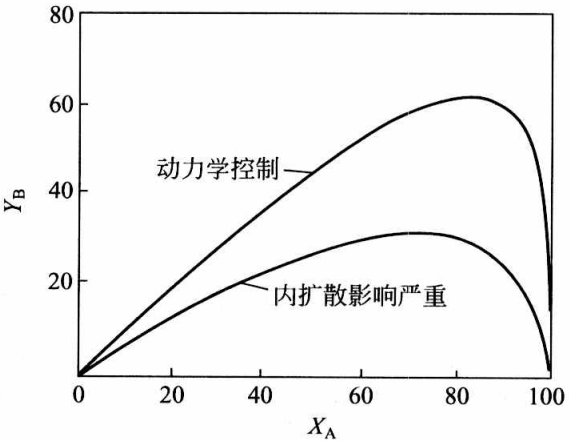
\includegraphics[width=\linewidth]{figures/fig6.7.png}
                \caption{内扩散对连串反应收率的影响}
            \end{figure}
        \end{minipage}

\end{frame}


\section{多相催化反应过程中扩散影响的判定}


\begin{frame}
    \frametitle{外扩散的主要影响因素}
    外扩散是反应物从流体主体传递到催化剂外表面的过程（或产物反向传递的过程）。其速率主要受流体力学条件和物理性质控制，与催化剂本身的化学反应特性无关。

    \bigskip

    \begin{minipage}{0.28\linewidth}
        \[
            \eta_{\mathrm{X}}=1 /(1+D a)
        \]
        \[
            D a=k_{\mathrm{W}} / k_{\mathrm{G}} a_{\mathrm{m}}
        \]
        \[
            j_{\mathrm{D}}=\frac{k_{\mathrm{G}} \rho}{G}(S c)^{2 / 3}
        \]
        \[
            S_{c}=\mu / \rho D
        \]
    \end{minipage}\hfill
    \begin{minipage}{0.68\linewidth}
        \begin{itemize}
          \item 质量流速($G$)：最核心、最直接的操作变量
          \item 颗粒粒径($d_p$)：关系复杂
          \item 粘度 ($\mu$)：粘度越大，传质阻力越大，$k_\mathrm{G}$越小
          \item 密度 ($\rho$)：影响雷诺数，从而影响流动状态
          \item 扩散系数 ($D$)：取决于物系和温度
        \end{itemize}
    \end{minipage}
    
\end{frame}


\begin{frame}
    \frametitle{各因素影响总结表}
    \begin{table}
        \centering
        \begin{tabularx}{\textwidth}{cXX}
            \bottomrule
            影响因素 & 如何影响外扩散速率 & 备注 \\ \hline
            质量流速($G$) & 提高流速，$Re$增大，$k_\mathrm{G}$显著提高。 & 判断外扩散控制：改变流速看反应速率是否变化。 \\ 
            颗粒粒径($d_p$) & 关系复杂。一般地，粒径减小，比表面积增大，但$k_\mathrm{G}$可能略微减小或不变。总体效应需具体计算。 & 与内扩散不同，粒径不是控制外扩散的主要手段。 \\ 
            流体粘度($\mu$) & 粘度增大，$Re$减小，$Sc$增大，导致$k_\mathrm{G}$减小。 & 高温通常可降低液体粘度。 \\
            流体密度 ($\rho$) & 直接使质量流速$G$增大，从而显著提高 $Re$ & 提高压力会显著增加密度 \\ 
            扩散系数 ($D$) & $D$增大，$Sc$减小，$k_\mathrm{G}$增大。 & 温度升高，$D$增大。\\\toprule
        \end{tabularx}
    \end{table}
\end{frame}


\begin{frame}
    \frametitle{如何判断及消除外扩散影响：流速实验}
        \bigskip
        \begin{minipage}{0.48\linewidth}
            \begin{figure}[htpb]
                \centering
                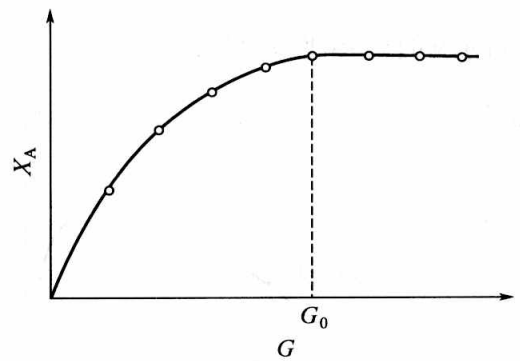
\includegraphics[width=\linewidth]{figures/fig6.8.png}
                \caption{流体质量速度对转化率的影响}
            \end{figure}            
        \end{minipage}\hfill
        \begin{minipage}{0.48\linewidth}
            \begin{itemize}
                \item 流体质量速度$G$，对外扩散有显著影响
                \item 保证在其他条件（如温度、反应物浓度、空时）相同的前提下，改变$G$以观察其对多相催化反应的影响。
                \item 当流体质量速度超过某一数值$G_0$时，出口转化率不再改变，外扩散对反应过程已无影响。
            \end{itemize}
        \end{minipage}

\end{frame}


\begin{frame}
    \frametitle{流速实验：实验室研究与工业化生产之间的矛盾}
    通过改变流体的质量速度以考察外扩散过程的影响，是多相催化反应动力学研究常采用的方法。实际生产的反应器难以采用上述方法。
    \begin{table}
        \centering
        \caption{实验室 vs. 工业化}
        \begin{tabularx}{\textwidth}{cXX}
            \bottomrule
             & 实验室反应器 & 工业反应器 \\ \hline
            目标 & 获取本征动力学数据，理解机理 & 经济、安全、稳定地生产产品 \\ 
            规模 & 小（克级催化剂，毫升/分钟流量） & 大（吨级催化剂，吨/小时流量） \\ 
            流速调节 & \bf{容易且成本极低} & \bf{困难且成本极高} \\
            主要约束 & 数据的准确性 & 经济性、安全性、操作性 \\ \toprule
        \end{tabularx}
    \end{table}

\end{frame}


\begin{frame}
    \frametitle{外扩散影响的判定：表观反应速率$\mathscr{R}_{\mathrm{A}}^{*}$}

    若能测得表观反应速率$\mathscr{R}_{\mathrm{A}}^{*}$，所进行的为$\alpha$级反应时，则可用下列判据来判定气相主体与催化剂外表面的浓度差是否可以忽略不计
    \[
        \frac{\mathscr{R}_{\mathrm{A}}^{*} L}{c_{\mathrm{AG}} k_{\mathrm{G}}}<\frac{0.15}{\alpha}
    \]
    气相与催化剂外表面间的温度差则可按下列判据来判断是否可以忽略
    \[
        \frac{L \mathscr{R}_{\mathrm{A}}^{*}\left(-\Delta H_{\mathrm{r}}\right)}{h_{\mathrm{S}} T_{\mathrm{G}}}<0.15 \frac{R T_{\mathrm{G}}}{E} 
    \]
    如符合上式，忽略相间温度差而造成反应速率的偏差不会大于5\%。

\end{frame}


\begin{frame}
    \frametitle{内扩散影响因素}

    内扩散有效因子是梯尔模数$\phi$的函数
    \[
        \phi=\frac{V_{\mathrm{p}}}{a_{\mathrm{p}}} \sqrt{\frac{k_{\mathrm{p}}}{D_{\mathrm{e}}}}
    \]
    当催化剂的组成和成型方法，以及反应的温度和反应物系的组成均一定时，仅取决于催化剂的颗粒粒度，因此，改变粒度进行实验，可以检验内扩散的影响程度。

    设所进行的是$\alpha$级不可逆反应，当外扩散影响已消除时，则其宏观反应速率可表示为
    \[
        \mathscr{R}_{\mathrm{A}}^{*}=-\frac{1}{W} \frac{\mathrm{d} N_{\mathrm{A}}}{\mathrm{d} t}=k_{\mathrm{W}} \eta c_\mathrm{AG}^ \alpha
    \]
    现有颗粒半径分别为$R_1$、$R_2$两种尺寸的同种催化剂床层，其反应条件维持相同，则反应速率之比为
    \[
        \frac{\mathscr{R}_{\mathrm{A} 1}^{*}}{\mathscr{R}_{\mathrm{A} 2}^{*}}=\frac{k_{\mathrm{W}} \eta_{1} c_{\mathrm{AG}}^{\alpha}}{k_{\mathrm{W}} \eta_{2} c_{\mathrm{AG}}^{\alpha}}=\frac{\eta_{1}}{\eta_{2}} 
    \]

\end{frame}


\begin{frame}
    \frametitle{内扩散影响因素}

    \begin{itemize}
        \item 不存在内扩散影响时        
        \[
            \mathscr{R}_{\mathrm{A} 1} = \mathscr{R}_{\mathrm{A} 2}
        \]
        \item 内扩散影响严重时，反应速率与颗粒半径成反比。
        \[
            \frac{\mathscr{R}_{\mathrm{A} 1}^{*}}{\mathscr{R}_{\mathrm{A} 2}^{*}}=\frac{\eta_{1}}{\eta_{2}}=\frac{\phi_{2}}{\phi_{1}}=\frac{R_{2}}{R_{1}}
        \]        
    \end{itemize}
    一般情况下，反应速率总是随颗粒尺寸的增大而减小的，依此原理，在催化剂床层中装填同样形状但粒度不同的同一种催化剂，通入反应气体，在相同反应条件下测定其反应速率，检验内扩散的影响程度。

\end{frame}


\begin{frame}
    \frametitle{内扩散影响的判定：粒度实验}
        \begin{minipage}{0.44\linewidth}
            \begin{figure}[htpb]
                \centering
                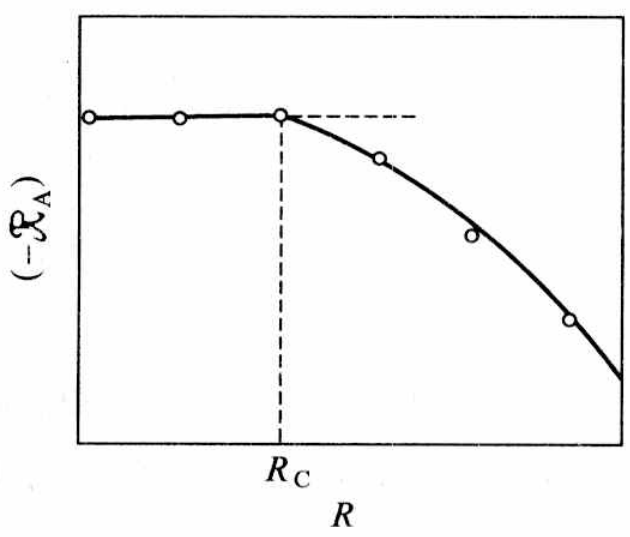
\includegraphics[width=\linewidth]{figures/fig6.9.png}
                \caption{催化剂半径对反应速率的影响}
            \end{figure}    
        \end{minipage}\hfill
        \begin{minipage}{0.48\linewidth}
            \begin{itemize}
                \item 反应速率将随粒度减小而增加。
                \item 当粒度减小到某一尺寸后，再减小粒度对反应速率即不再有影响
                \item 对$R<R_\mathrm{c}$的催化剂颗粒，内扩散阻力对反应过程可以认为没有影响。
                \item 内扩散不发生影响的粒度，与温度有关，也与浓度有关（一级反应例外）。
            \end{itemize}
        \end{minipage}

\end{frame}


\begin{frame}
    \frametitle{内扩散影响的判定：粒度实验}
    \[
        \eta = \frac{1}{\phi}=\frac{1}{\frac{V_{\mathrm{p}}}{a_{\mathrm{p}}} \sqrt{\frac{k_{\mathrm{p}}}{D_{\mathrm{e}}}}}
    \]
    \begin{itemize}
        \item 反应温度越高，消除内扩散影响所要求的粒度越小。
    \end{itemize}
    \[
        \text{对于$\alpha$级反应，} \eta=\frac{\sqrt{2 D_{\mathrm{e}}}}{L \sqrt{k_{\mathrm{p}}} c_{\mathrm{AS}}^\alpha}\left[\int_{0}^{c_{\mathrm{AS}}} c_{\mathrm{A}}^\alpha \mathrm{d} c_{\mathrm{A}}\right]^{1 / 2}=\frac{1}{L} \sqrt{\frac{2 D_{\mathrm{e}}}{(\alpha+1) k_{\mathrm{p}} c_\mathrm{AS}^{\alpha - 1}}}
    \]
    \begin{itemize}
        \item 浓度$c_{\mathrm{AS}}$越高，消除内扩散影响所要求的粒度越小。
    \end{itemize}
    若在高温、高反应物浓度下，已判明消除了内、外扩散的影响。那么，可以保证在低温、低反应物浓度时也不会有内、外扩散的影响，反应物的级数为负数时为例外。

\end{frame}


\begin{frame}
    \frametitle{内扩散影响的判定：表观反应速率$\mathscr{R}_{\mathrm{A}}^{*}$}
    若反应系统已排除外扩散阻力影响，对于一级反应，实测表观反应速率$\mathscr{R}_{\mathrm{A}}^{*}$为
    \[
        \mathscr{R}_{\mathrm{A}}^{*}=\eta k_{\mathrm{p}} c_{\mathrm{AG}}
    \]
    如果$k_{\mathrm{p}}$已知，显然可由上式求$\eta$来判断内扩散的影响程度。但是，在实际工业生产中，往往本征反应速率常数$k$和级数$n$是未知的，在这种情况下，可以通过计算无量纲参数$\phi^2\eta$来判断。$\mathscr{R}_{\mathrm{A}}^{*}=\eta k_{\mathrm{p}} c_{\mathrm{AG}}$代入$\phi = L\sqrt{\frac{k_\mathrm{p}}{D_{\mathrm{e}}}}$，得
    \[
        \phi=L \sqrt{\frac{\mathscr{R}_{\mathrm{A}}^{*}}{\eta c_{\mathrm{AG}}D_{\mathrm{e}}}}
    \]
    \[
        \phi^2\eta = \frac{L^2 \mathscr{R}_{\mathrm{A}}^{*}}{c_{\mathrm{AG}}D_{\mathrm{e}}}
    \]    

\end{frame}


\begin{frame}
    \frametitle{内扩散影响的判定：表观反应速率$\mathscr{R}_{\mathrm{A}}^{*}$}
    \begin{figure}[htpb]
        \centering
        
\includegraphics[width=.6\linewidth]{fig6.5}
    \end{figure}
    \begin{itemize}
        \item $\phi \leqslant 0.4$时，$\eta \approx 1$，内扩散阻力影响可忽略。此时$\phi^2\eta <0.16$；
        \item $\phi \geqslant 3$时，内扩散阻力有明显影响，此时$\eta \approx 1/\phi$，$\phi^2\eta \geqslant 3$。
    \end{itemize}
\end{frame}

\begin{frame}
    \frametitle{内扩散影响的判定}

    上述结论是对一级反应导出的，亦可用于非一级反应，但$\phi$的定义要修改。
    
    定义一普遍化梯尔模数：
    \[
        \phi^{2}=\frac{L^{2} k_{\mathrm{p}}\left[f(c_{\mathrm{AG}})\right]^{2}}{2 D_{\mathrm{e}} \int_{c_{\mathrm{AC}}}^{c_{\mathrm{AG}}} f(c_{\mathrm{A}}) \mathrm{d} c_{\mathrm{A}}}
    \]
    \[
        \phi^{2} \eta=\frac{\mathscr{R}_{\mathrm{A}}^{*} L^{2} f(c_{\mathrm{AG}})}{2 D_{\mathrm{e}} \int_{c_{\mathrm{AC}}}^{c_{\mathrm{AG}}} f(c_{\mathrm{A}}) \mathrm{d} c_{\mathrm{A}}}
    \]

\end{frame}


\begin{frame}[t]
    \frametitle{}
    \begin{example}
        进行一气固相催化反应动力学的研究，反应为\ch{A + B -> R}，反应温度为200℃，A的分压$p_\mathrm{A} =\ $\SI{0.051}{MPa}，B的分压$p_\mathrm{B} =\ $\SI{0.253}{MPa}，B组分过量，该反应可看作一级反应。所用催化剂颗粒的平均直径为\SI{0.14}{cm}，催化剂颗粒密度为\SI{1.39}{g/cm^3}，测得表观反应速率$\mathscr{R} =$\SI{0.032}{mol/(h.g)}，若有效扩散系数$D_\mathrm{e} =$\SI{0.0248}{cm^2/s}，试估计内部传递的影响。
        \tcblower
    \pause
    \[
        c_{\mathrm{AG}}=\frac{p_{\mathrm{A}}}{R T}=\frac{0.051}{8.314 \times 473}=1.29 \times 10^{-5} \mathrm{~mol} / \mathrm{cm}^{3}
    \]
    \[
        \mathscr{R}=\frac{0.032}{3600} \times 1.39=1.24 \times 10^{-5} \mathrm{~mol} /(\mathrm{s} \cdot \mathrm{cm}^{3})
    \]
    \[
        \Phi^{2} \eta= \frac{r_{\mathrm{p}}^{2}\mathscr{R}}{c_{\mathrm{AG}} D_{\mathrm{e}}}= \frac{0.07^{2}\times 1.24 \times 10^{-5}}{1.29 \times 10^{-5} \times 0.0248}=0.19<1.44 \quad \text{内扩散影响可忽略}
    \]
    \end{example}
\end{frame}


\section{扩散干扰下的动力学假象}

\begin{frame}
    \frametitle{外扩散干扰下的动力学假象}

    在进行多相催化反应的动力学实验时，需要排除内、外扩散的影响，以获得反映化学现象本质的信息，如反应级数和反应活化能等。如在扩散干扰下作实验测定，将得不到这些动力学参数的本征值。

    若在处于外扩散控制的条件下进行多相催化反应的动力学实验测定，无论该反应的本征速率方程是何种形式，根据实验所得的反应速率数据与反应物浓度相关联的结果均成线性关系。这就是说处于外扩散控制区的任何反应表观上都变成了一级反应。    
    \[
        N_\mathrm{A} = k_\mathrm{G}a_\mathrm{m}(c_\mathrm{AG} - c_\mathrm{AS})
    \]
    因此，若不注意外扩散影响的排除，就有可能得出某一反应为一级反应的错误结论。特别是做实验室规模的实验测定时更应格外小心，因为实验室反应器所用的流体质量速度往往较低，从而相间传递的影响可能相当显著。

\end{frame}


\begin{frame}
    \frametitle{内扩散干扰下的动力学假象}

    外扩散阻力可以忽略时，$\alpha$级不可逆反应的反应速率可表示为
    \[
        \mathscr{R}_{\mathrm{A}}^{*}=\eta k_{\mathrm{p}} c_{\mathrm{AG}}^\alpha
    \]
    内扩散有影响的条件下，测得如下的速率方程
    \[
        \mathscr{R}_{\mathrm{A}}^{*}=k_{\mathrm{a}} c_{\mathrm{AG}}^{\alpha_\mathrm{a}}
    \]
    按理说两式是等同的，但反应级数不同，1式中的$\alpha$称为本征反应级数，而2式中的$\alpha_\mathrm{a}$则叫做表观反应级数。$\alpha$是该反应所固有的性质，是一个定值；而$\alpha_\mathrm{a}$则随内扩散影响程度的不同而改变。下面将要说明和两者之间的关系。

\end{frame}


\begin{frame}
    \frametitle{内扩散干扰下的动力学假象}

    对$\mathscr{R}_{\mathrm{A}}^{*}=\eta k_{\mathrm{p}} c_{\mathrm{AG}}^\alpha$，$\mathscr{R}_{\mathrm{A}}^{*}=k_{\mathrm{a}} c_{\mathrm{AG}}^{\alpha_\mathrm{a}}$取对数，得
    \[
        \ln \mathscr{R}_{\mathrm{A}}^{*}=\ln \eta+\ln k_{\mathrm{p}}+\alpha \ln c_{\mathrm{AG}}
    \]
    \[
        \ln \mathscr{R}_{\mathrm{A}}^{*}= \ln k_{\mathrm{a}}+\alpha_\mathrm{a} \ln c_{\mathrm{AG}}
    \]
    等温下求导，得
    \[
        \begin{aligned}
             \frac{\mathrm{d} \ln \mathscr{R}_{\mathrm{A}}^{*}}{\mathrm{~d} \ln c_{\mathrm{AG}}}&=\alpha+\frac{\mathrm{d} \ln \eta}{\mathrm{d} \ln c_{\mathrm{AG}}}\\
             \frac{\mathrm{d} \ln \mathscr{R}_{\mathrm{A}}^{*}}{\mathrm{~d} \ln c_{\mathrm{AG}}}&=\alpha_{\mathrm{a}}
        \end{aligned}
    \]
    两式合并后有
    \[
        \alpha_{\mathrm{a}}=\alpha+\frac{\mathrm{d} \ln \eta}{\mathrm{d} \ln c_{\mathrm{AG}}}=\alpha+\frac{\mathrm{d} \ln \eta}{\mathrm{d} \ln \phi} \frac{\mathrm{d} \ln \phi}{\mathrm{d} \ln c_{\mathrm{AG}}}
    \]

\end{frame}


\begin{frame}
    \frametitle{内扩散干扰下的动力学假象}

    若催化剂为薄片形,$\alpha$级反应的梯尔模数$\phi$为
    \[
        \phi=L \sqrt{\frac{k_{\mathrm{p}}}{2 D_{\mathrm{e}}}} \frac{c_\mathrm{AG}^{\alpha}}{\left[\int_{0}^{c_{\mathrm{AG}}} c_{\mathrm{A}}^{\alpha} \mathrm{d} c_{\mathrm{A}}\right]^{1 / 2}}=L\left[\frac{(\alpha+1) k_{\mathrm{p}}}{2 D_{\mathrm{e}}}\right]^{1 / 2} c_{\mathrm{AG}}^{(\alpha-1) / 2}
    \]
    两边取对数，然后求导得
    \[
        \frac{\mathrm{d} \ln \phi}{\mathrm{d} \ln c_{\mathrm{AG}}} =(\alpha-1) / 2
    \]
    那么
    \[
        \alpha_{\mathrm{a}}=\alpha+\frac{(\alpha-1)}{2} \times \frac{\mathrm{d} \ln \eta}{\mathrm{d} \ln \phi}
    \]
    

\end{frame}


\begin{frame}
    \frametitle{内扩散干扰下的动力学假象}

    \begin{itemize}
        \item 当内扩散影响不存在时$\eta =1$，        
        \[
            \alpha_{\mathrm{a}}=\alpha \qquad
        \]
        表观反应级数等于本征值。
        \item 若内扩散的影响严重，则$\eta =1/\phi$，因而有$\frac{\mathrm{d} \ln \eta}{\mathrm{d} \ln \phi} = -1$，        
        \[
            \alpha_{\mathrm{a}}= \frac{(\alpha+1)}{2}
        \]        
        本征反应级数为0、1及2时，表观反应级数分别为0.5，1及1.5。

        只有一级反应两者值相同，原因是内扩散对一级反应的影响与浓度无关。
        
        其他反应则随着内扩散干扰程度的不同，反应级数从$(\alpha+1)/2$至$\alpha$的范围内改变。
    \end{itemize}

\end{frame}


\begin{frame}
    \frametitle{内扩散对反应活化能的影响}

    设表观反应速率常数$k_\mathrm{a}$与温度的关系符合阿伦尼乌斯方程，且表观活化能为$E_\mathrm{a}$，则将$\mathscr{R}_{\mathrm{A}}^{*}=k_{\mathrm{a}} c_{\mathrm{AG}}^{\alpha_\mathrm{a}}$两边取对数，并对$1/T$求导可得
    \[
        \frac{\mathrm{d} \ln \mathscr{R}_{\mathrm{A}}^{*}}{\mathrm{~d}(1 / T)}=\frac{\mathrm{d} \ln k_{\mathrm{a}}}{\mathrm{d}(1 / T)}=-\frac{E_{\mathrm{a}}}{R}
    \]
    若本征反应速率常数$k_\mathrm{p}$与温度的关系亦可用阿伦尼乌斯方程表示，且本征活化能为$E$，则将式$\mathscr{R}_{\mathrm{A}}^{*}=\eta k_{\mathrm{p}} c_{\mathrm{AG}}^\alpha$对$1/T$求导可得
    \[
        \frac{\mathrm{d} \ln \mathscr{R}_{\mathrm{A}}^{*}}{\mathrm{~d}(1 / T)}=\frac{\mathrm{d} \ln k_{\mathrm{p}}}{\mathrm{d}(1 / T)}+\frac{\mathrm{d} \ln \eta}{\mathrm{d}(1 / T)}=\frac{-E}{R}+\frac{\mathrm{d} \ln \eta}{\mathrm{d}(1 / T)}
    \]
    两式合并并作适当改写，得
    \[
        E_{\mathrm{a}}=E-R \frac{\mathrm{d} \ln \eta}{\mathrm{d} \ln \phi} \times \frac{\mathrm{d} \ln \phi}{\mathrm{d}(1 / T)}
    \]

\end{frame}


\begin{frame}
    \frametitle{内扩散对反应活化能的影响}

    将$\alpha$级反应的梯尔模数$\phi$的表达式两边取对数，然后对$1/T$求导，忽略温度对$D_\mathrm{e}$的影响时有
    \[
        \frac{\mathrm{d} \ln \phi}{\mathrm{d}(1 / T)}=\frac{1}{2} \frac{\mathrm{d} \ln k_{\mathrm{p}}}{\mathrm{d}(1 / T)}=-\frac{E}{2 R}
    \]
    则
    \[
        E_{\mathrm{a}}=E+\frac{E}{2} \times \frac{\mathrm{d} \ln \eta}{\mathrm{d} \ln \phi}
    \]
    这便是表观活化能与本征活化能的关系式。

    表观活化能系随着内扩散干扰的程度不同而改变。
    \begin{itemize}
        \item $\phi$值甚小时，$\eta \approx 1$，此时表观活化能等于本征活化能。
        \item $\phi$值甚大时，$\frac{\mathrm{d} \ln \eta}{\mathrm{d} \ln \phi} = -1$，$E_{\mathrm{a}}=E/2$。即内扩散影响严重时，表观活化能仅为本征活化能的一半。
    \end{itemize}

\end{frame}


\begin{frame}
    \frametitle{内扩散对反应活化能的影响}

        \begin{minipage}{0.4\linewidth}
            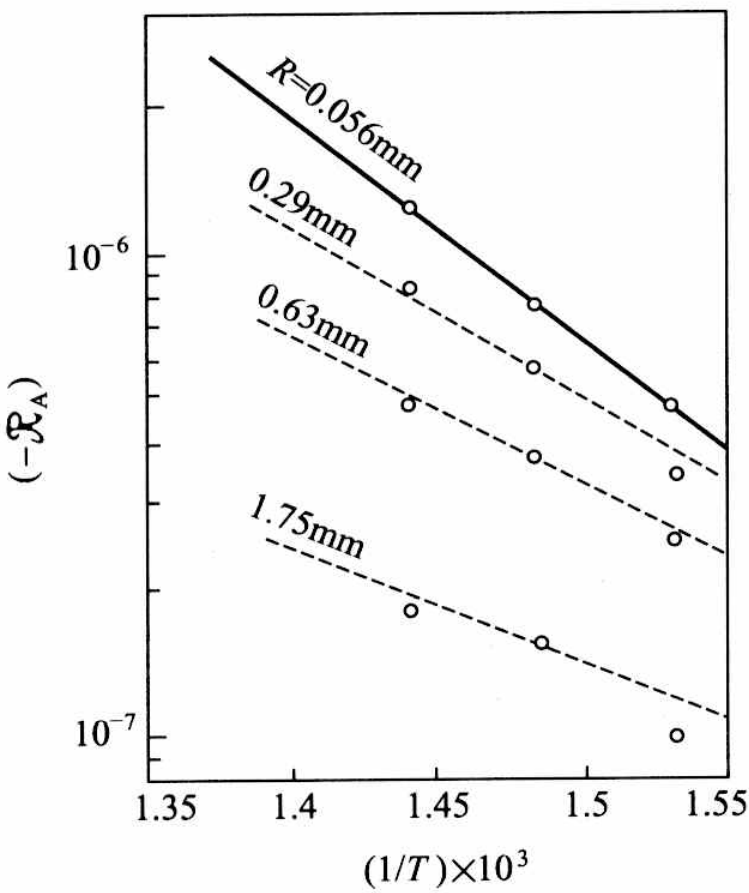
\includegraphics[width=\linewidth]{figures/fig6.10.png}
        \end{minipage}\hfill
        \begin{minipage}{0.58\linewidth}
            \begin{itemize}
                \item 由于催化剂粒度的不同，因而内扩散的影响也不相同。
                \item 对于同一粒度的实验点均能落在同一条直线上。根据直线的斜率便可确定反应活化能。
                \item 催化剂的粒度越小，直线的斜率越大。
                \item 反应的表观活化能系随催化剂粒度的增加而减小，亦即随内扩散影响的增大而减小。
            \end{itemize}
        \end{minipage}

\end{frame}


\begin{frame}
    \frametitle{扩散对多相催化反应活化能的影响}

        \begin{minipage}{0.56\linewidth}
            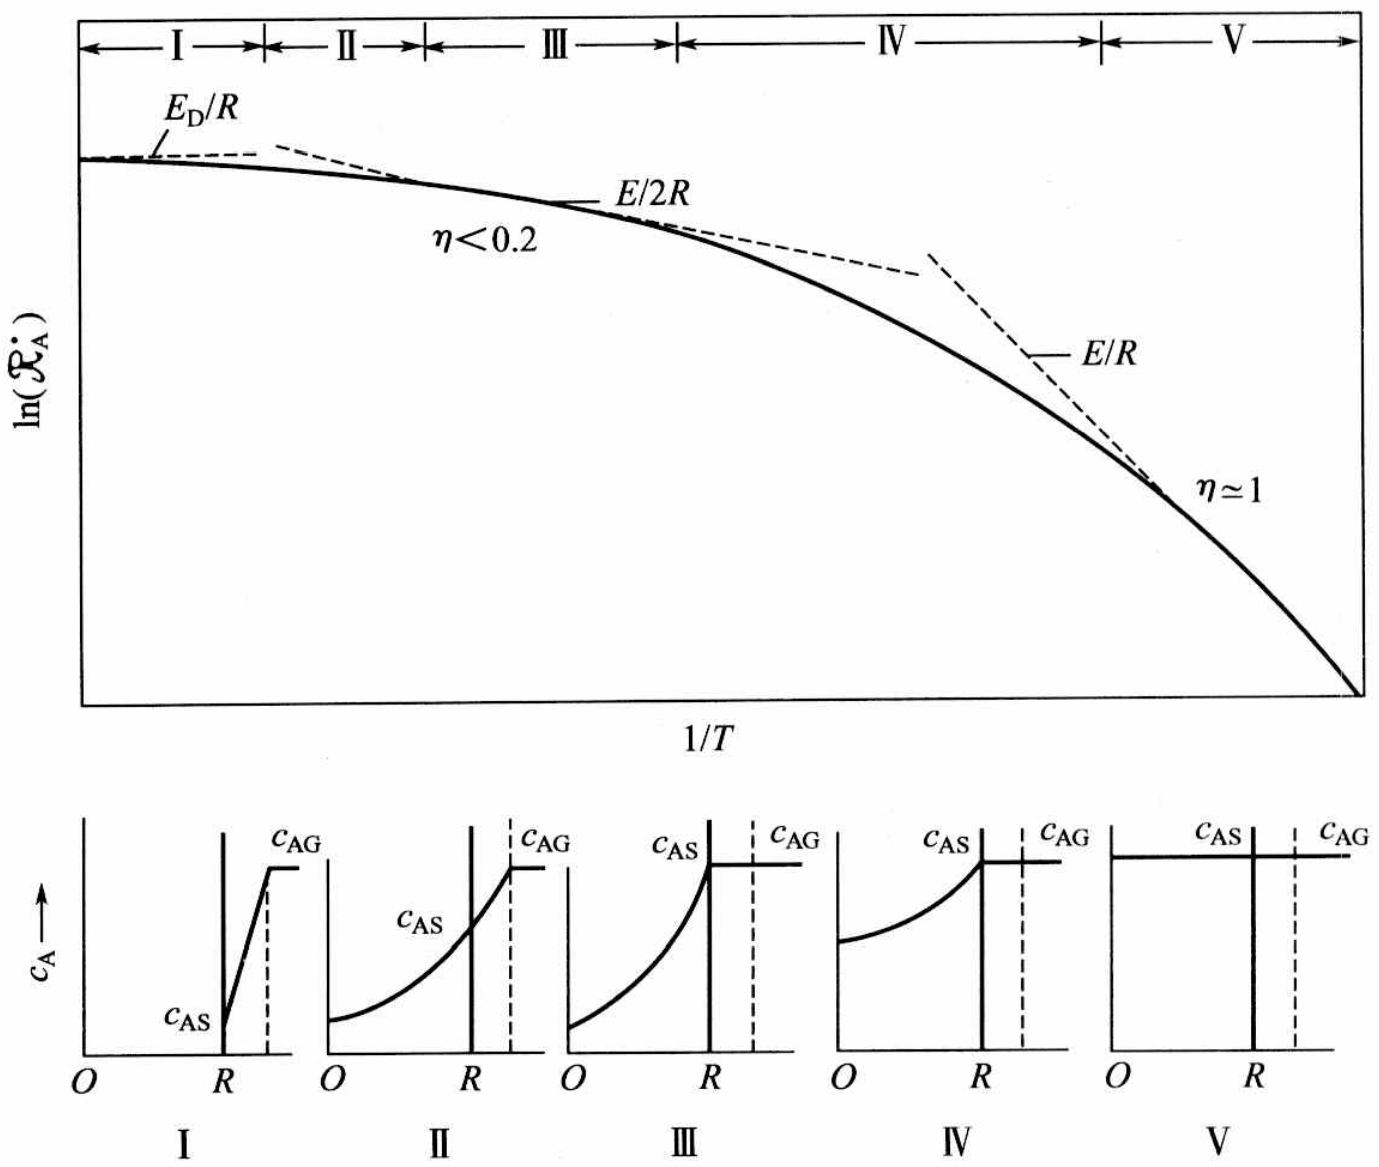
\includegraphics[width=\linewidth]{figures/fig6.11.png}
        \end{minipage}\hfill
        \begin{minipage}{0.4\linewidth}
            \begin{itemize}
                \item[I区] 高温区，外扩散控制
                
                活化能$E_\mathrm{D}$几乎为零
                \item[II区] 内外扩散过渡区
                
                活化能随温度而变
                \item[III区] 强内扩散区
                
                活化能近于常数，为$E/2$
                \item[IV区] 内扩散动力学过渡区
                
                活化能随$T$变化更显著
                \item[V区] 动力学控制区
                
                低温区，有效因子接近1
            \end{itemize}
        \end{minipage}
    

\end{frame}


\begin{frame}
    \frametitle{扩散对多相催化反应活化能的影响}

    \begin{enumerate}
        \item 多相催化反应的活化能严格说来并非定值，而是温度的函数。
        \item 只有在某些温度范围内可近似地认为是常数
            \begin{itemize}
                \item[\bullet] 外扩散控制区
                \item[\bullet] 强内扩散区
                \item[\bullet] 动力学控制区
            \end{itemize}
        \item 以上三个区的活化能值依次增高
        \item 这种差别是由于温度对化学反应和传质过程的影响不同
        \item 就一个反应而言，温度的改变会使过程从一个区转到另一个区
        \item 随着温度的降低，扩散影响趋于减弱。
    \end{enumerate}

\end{frame}    
	


\end{document}